\section{Application to proplyd bowshocks}
\label{sec:application}


The density distribution of the photoevaporated flow can be determined using the steady state continuity equation and assuming that almost all ionizing photons are absorbed at the IF 
\citep{HA:1998} and ignoring dust absorption, can be found that

\begin{align}
N(r_{IF},\theta) = N_0 \cos^{0.5}\theta
\label{eq:nprop}
\end{align}

Neverthless, we should not restrict to the 0.5 index in equation (\ref{eq:nprop}). We may generalize this relation as follows:

\begin{align}
n(r_{IF},\theta) = n_0 \cos^{k}\theta
\label{eq:ngen}
\end{align}

Where $k >0$ implies that the wind's density decays towards wings, when $k<0$ the wind's density incresases towards the wings and $k=0$
implies that the wind is isotropic.
In this generalization we are assuming that the inner wind is hemispheric, i.e. the density of the photoevaporated flow behind the source is zero, since equation
(\ref{eq:ngen}) leads to non realistic values for density when $\theta > \frac{\pi}{2}$



% Combining equations (6),(9)-(11) and (19)-(23) from \citep{Canto:1996} and (\ref{eq:nprop}), we can solve numerically for $R(\theta)$, which gives us the shell's shape. Also we can
%obtain a relation between $\theta$ and $\theta_1$

%\begin{align}
%\theta_1\cot\theta_1 = 1+ 2\beta I(\theta)\cot\theta - \frac{4}{5}\beta\left(1-\cos^{5/2}\theta\right)
%\label{eq:th1th}
%\end{align}

%Where $I(\theta)\equiv \int^\theta_0 \cos^{1/2}\theta\sin^2\theta~d\theta$. The solution of this integral is an incomplete elliptical integral of the second kind:

%\begin{align}
%\int^\theta_0 \cos^{1/2}\theta\sin^2\theta~d\theta = \frac{4}{5}E\left(\frac{\theta}{2}|2\right) - \frac{1}{5}\sin 2\theta\cos^{1/2}\theta
%\end{align}



%Although there is an analytical form for the radius of curvature, for $i\ne 0$ there is not an intuitive form for  $R'_c$. Plus, in practice, we are working with discret arrays, so, when transforming the shell's coordinates to the primed system, we almost certainly will miss the $\theta'=0$ point, which
%should allow us to estimate the radii $(R'_0,R'_c)$, the first with equation (\ref{eq:Rpar}) and the second with the mathematical definition of the radius of curvature using the primed coordinates. Insted, we estimate $R'_0$ as the projected radius with the value of $\theta'$ closest to zero, and
%$R'_c$ doing a least square fit to the points such as $\theta' \leq 45^\circ$. This restriction allows to obtain the best estimation of the radius of curvature at the nos of the shell. A lower cuttoff may undestimate $R'_c$ while higher cutoffs might be unaccurate, too.


 
\subsection{Observational data}

We measured the Characteristic radii in Orion Nebula proplyds from observations with the WPC2 camera from the Hubble Space Telescope (HST) using the narrow [OIII] filter. The original proposal were done by John Bally (The proposal ID is 5469). In figure \ref{fig:radii-measures-example}, we show the field where our proplyds sample lies with the measurements of each bow shock shape we made.

\subsection{Methodology}
\label{sec:methodology}
Using the DS9 SAO image tools, we marked the positions of the proplyds and \thC{}. For the shell's position, the marks were placed in the outer border of each shock. 
The number of marks used in each shell varies with shell's size, and with our confidence with our measurements.
Thus, we used few points in small bow shocks and/our the bow shock's outer shell is not well defined. The distance $D$ is measured as the distance between the position of \thC{} 
and each proplyd's position. The radius of curvature $R_c$ is measured as the radius of the 
best circle fit of all the data points taken for each proplyd's shell. Finally, we measure $R_0$ as the distance between the proplyd's position and the circle's border in the line which 
include the center of curvature.
To estimate the uncertainties of our measurements, we remove a fraction of the shell's marks, and made 10 sets of randomly chosen removed marks, and made the measurements again to 
see how much these subsamples deviates from the original data. Some examples are shown  in figure (\ref{fig:char-radii-obs}).  In the left side, for each source, 
the fit is done using all the shell points, while in the middle and the right we show two variations removing 2/3 of the points, but always keeping at least four. 
In the better observed shells such as 177-341 (top row), the circle
fits are relatively robust to removing points, resulting in little variation between the subsamples. 
But also there are cases where the variations between subsamples are more noticeable. Colums 3, 4 and 5 of table (\ref{tab:arc-fits}) represent the summary of all the measurements done. In colums 4 and 5, 
the radii $(R_0,R_c)$ are measured as the average of all subsamples, and the uncertainty as the standard deviation.

\section{Results}
\label{sec:results}
In figure (\ref{fig:conic-xi}) we show the theoretical conic curves. Most of the proplyds fit well 
with a elliptic-like conic shape and moderate to high degree of anisotropy of their wind.

Beneath the error margins, our measurements are consistent with \citet{Robberto:2005} for $R'_0/D$. From figure (\ref{fig:conic-xi}), we also
note that the LV4 measurements fits better with models where its photoevaporated flow is isotropic. The same is true with \citet{Robberto:2005} data.
The rest of the proplyds fit better with more anisotropic winds, which may explain why \citet{Robberto:2005} did not find a match between models
and data, since they only showed models where the interacting winds are isotropic.

With the data from figure \ref{fig:conic-xi}, we derived a set of models which assumes a given set of bow shock parameters $(\beta, i,\xi)$ and have agreement with the measurements of each proplyd. A given model predicts the no projected
distance $D$ for the proplyd and the non projected radius $R_0$. We summarize the results of the models in table \ref{tab:arc-fits}.

From this models also we can estimate the stellar ionizing flux required to have ionization balance with the photoevaporated flow. To do this estimation we used the measured ionization front radius and the photoevaporated flow density for each proplyd
and incorporated them into the models. The result is shown in figure \ref{fig:pressure} at top. We highlight the models which have agreement with ionization balance.
Also we can estimate the stagnation pressure of the photoevaporated flow. The result is shown in figure \ref{fig:pressure} at bottom. 
From this figures we can see that our models predict that for the farthest proplyds (169-338, 177-341 and 180-331) the stellar wind pressure is weaker than the estimated stagnation pressure. Since these bow shocks are stationary, we expect pressure
balance, so the stellar wind is not enough to guarantee pressure balance far from \thC{}

%Using the data from figure \ref{fig:conic-xi}, we estimate for each source the parameters $(\beta,i,\xi)$ (columns 7, 8 and 9 from table \ref{tab:arc-fits}). With this, is possible to estimate the non projected distances $(R_0,D)$ (columns 10 and 11).

%Using the data from table \ref{tab:arc-fits} along with the ionization front radius and photoevaporation flow density obtained from \citet{HA:1998} we measured the stagnation pressure at the bow shock's position, 
%and compare it with the expected pressure from the stellar wind at the distance $D$. 
%Since we expect equilibrium pressure in the bow shock surface, both pressures should be the same. The comparison is done in figure \ref{fig:pressure} (bottom).

%We also expect the stellar ionizing flux should be the required to balance the photoevaporated flux. We do
%the comparison in figure \ref{fig:pressure} (top). In both cases, the highlighted points represent the variations which have better agree with ionization balance and pressure balance, respctively.
 
%For the farthest proplyds, we can see that the estimated pressure is greater than the stellar wind pressure, even with the best fits. This suggests that at large distances, another source rather than the 
%stellar wind is the reponsible for mantaining the stationary bow shocks. 

\begin{figure*}
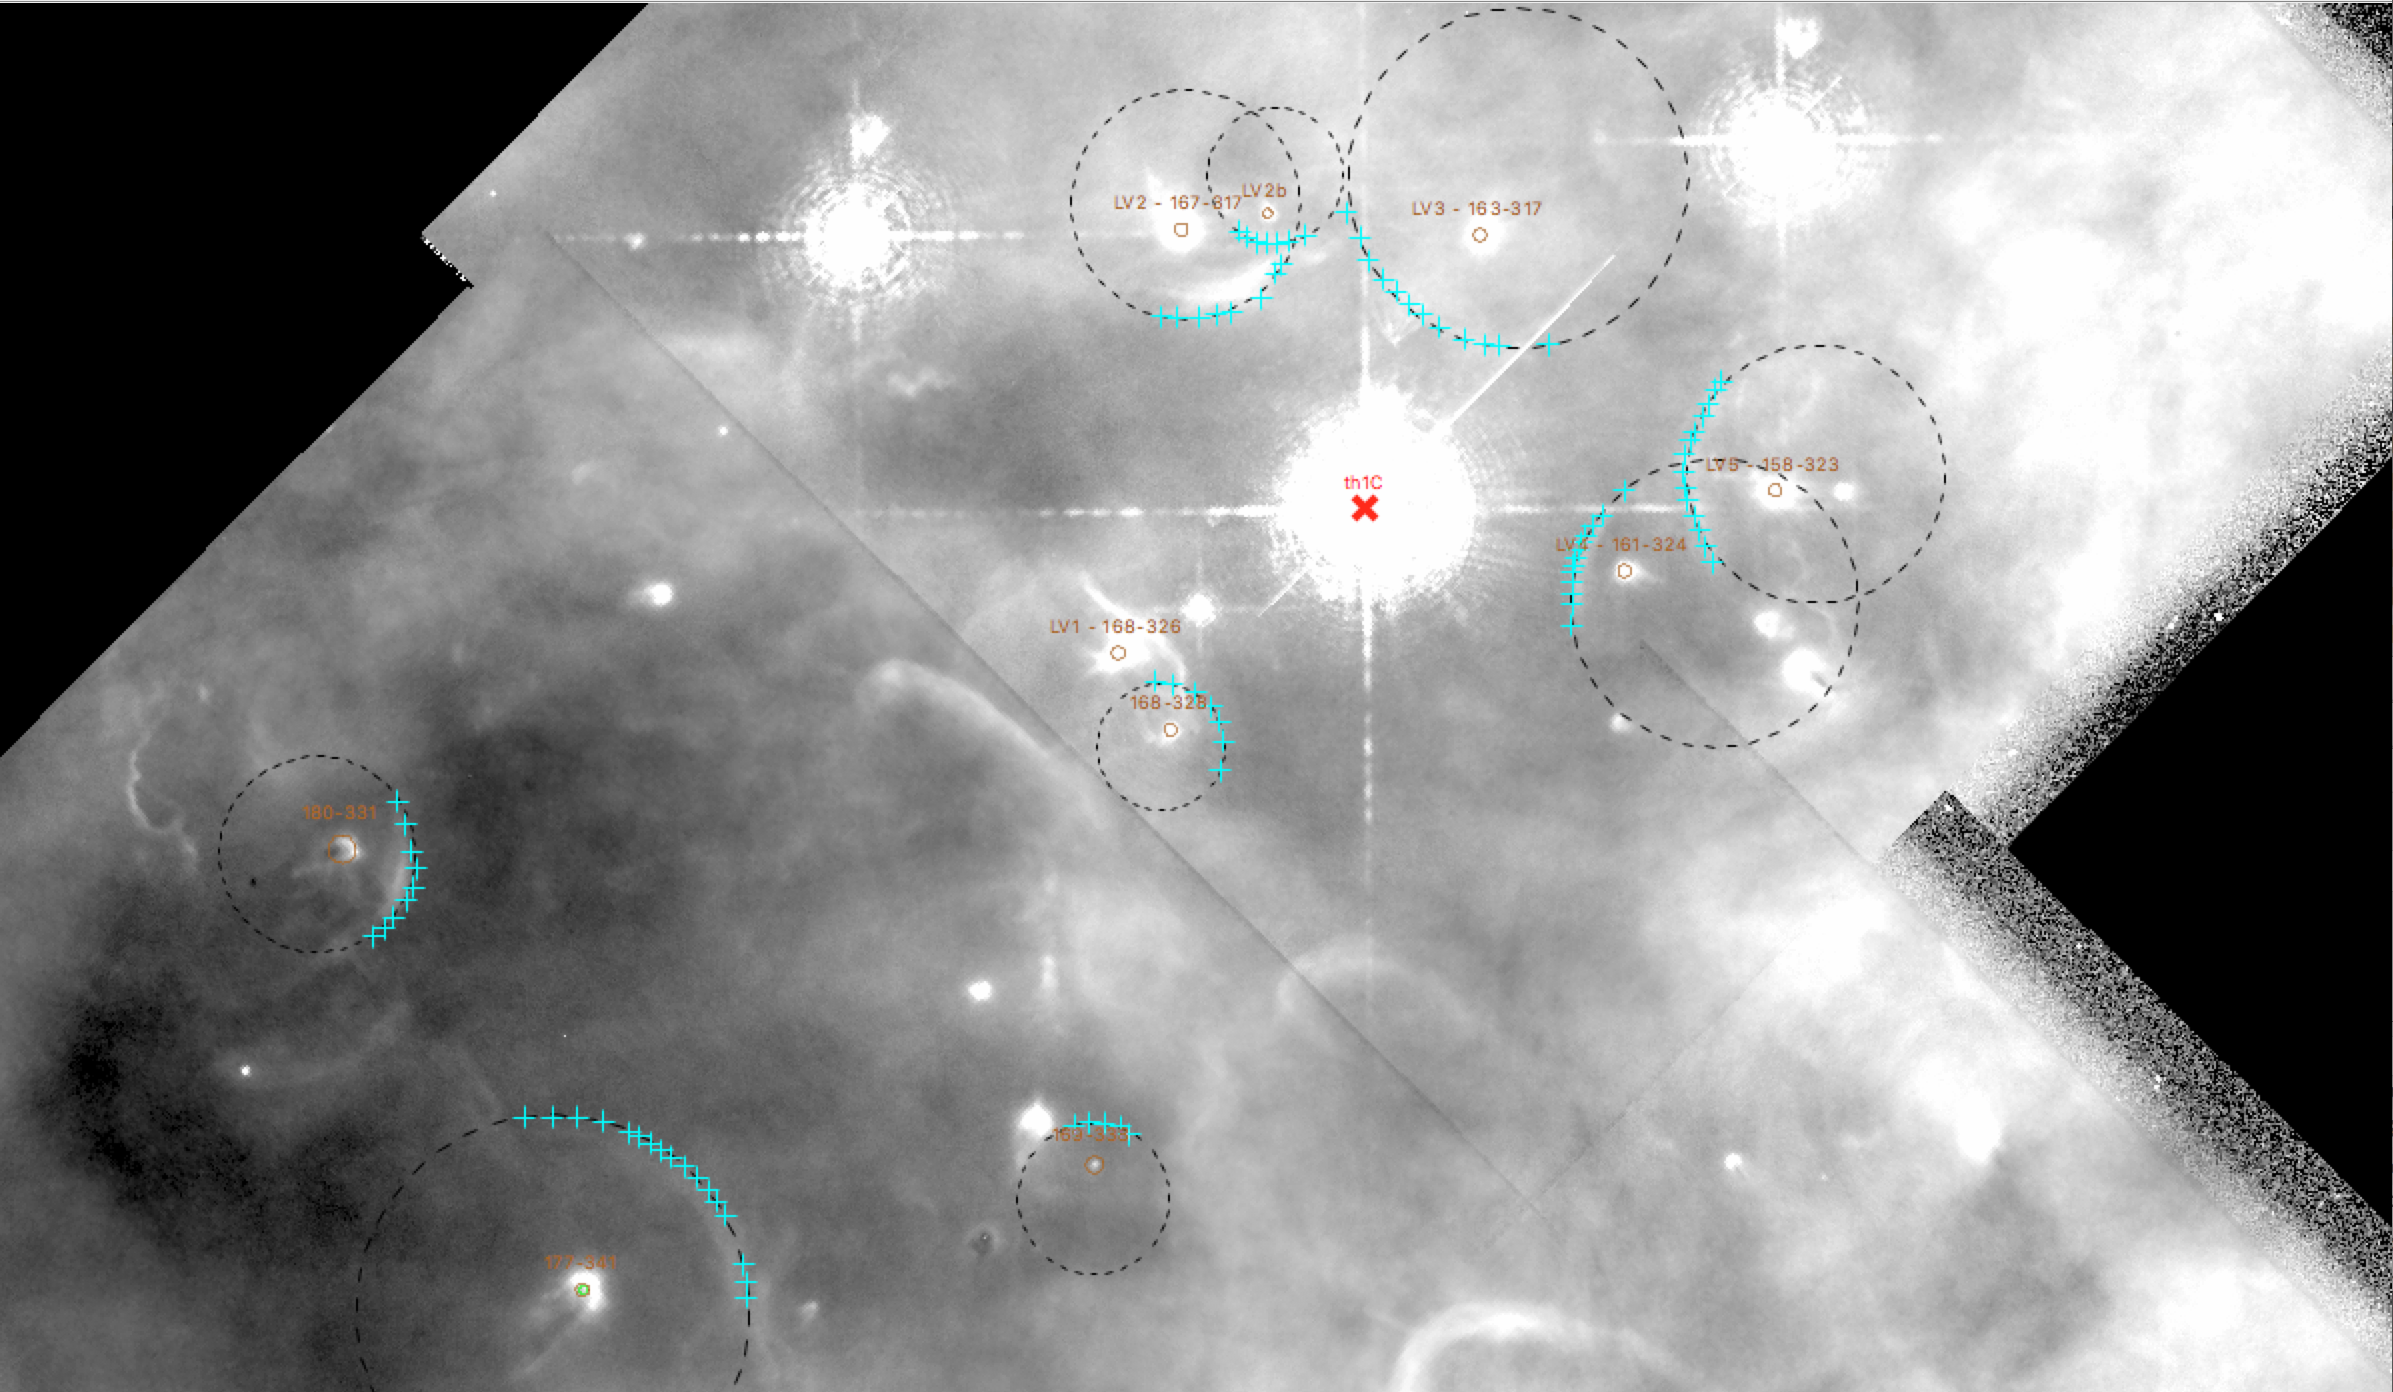
\includegraphics[width=\linewidth]{LV-full-field-annotated.png}
\caption{DS9 shell marks over ONC. The circles mark each proplys position, while the cyan crosses delineate each bow shock and the red X marks the position of $\theta^1 ~C~Ori$. 
The black circles only schematize a circle fit to each shell but they actually are not the real measurements.}
\label{fig:radii-measures-example}
\end{figure*}


%\begin{figure}
%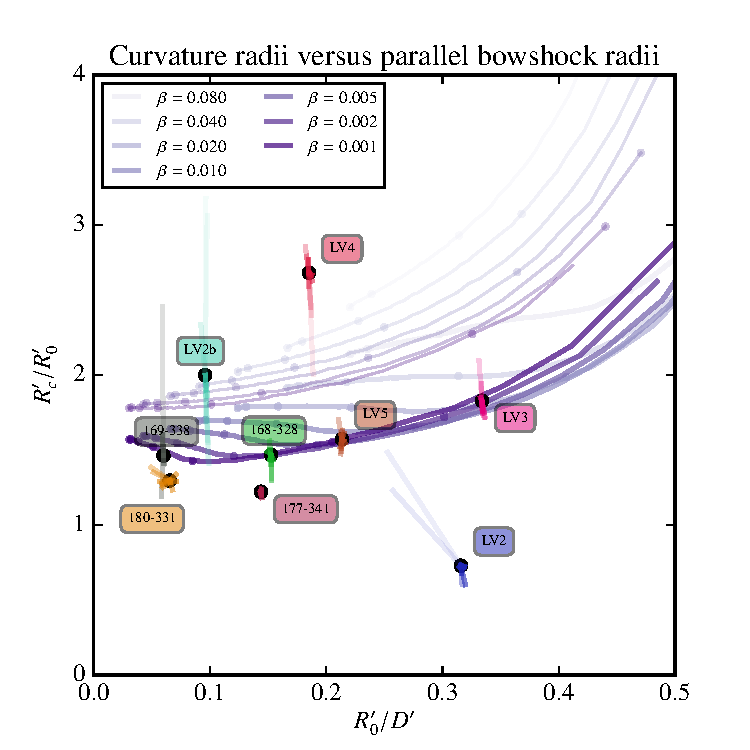
\includegraphics[width=\linewidth]{../../read-shapes/proplyd-shell-R0-Rc-cloud} 
%\label{fig:prop-shell-rad}
%\caption{Measurements of proplyd's characteristic radii $R_c$ and $R_0$. The curves represent a single bow shock with  fixed wind's momentum ratio $\beta$. 
%The dots represent separations in inclination of $15^{\circ}$. The semitransparent curves represent bow shocks which the inner wind is isotropic and the full colored 
%curves bow shocks which inner wind density decays as $\cos^{1/2}\theta$. The observational measurements are accompained with radial bars which represents the variations 
%with a fraction of the shell's marks removed. Proplyds with less data marks or high asymmetry show higher deviations in the measurements.
%Our measures match far better than \citep{Robberto:2005}, but our data tend to lie at high inclinations $i \gtrsim 45^\circ$, when we expected the opposite. Right side: The same
%}
%\end{figure}


\begin{figure*}
  \setkeys{Gin}{width=0.33\linewidth, trim=10 30 55 62.5}
\begin{tabular}{@{}c@{}c@{}c@{}}
 
All points & First sub-sample & Second sub-sample \\ 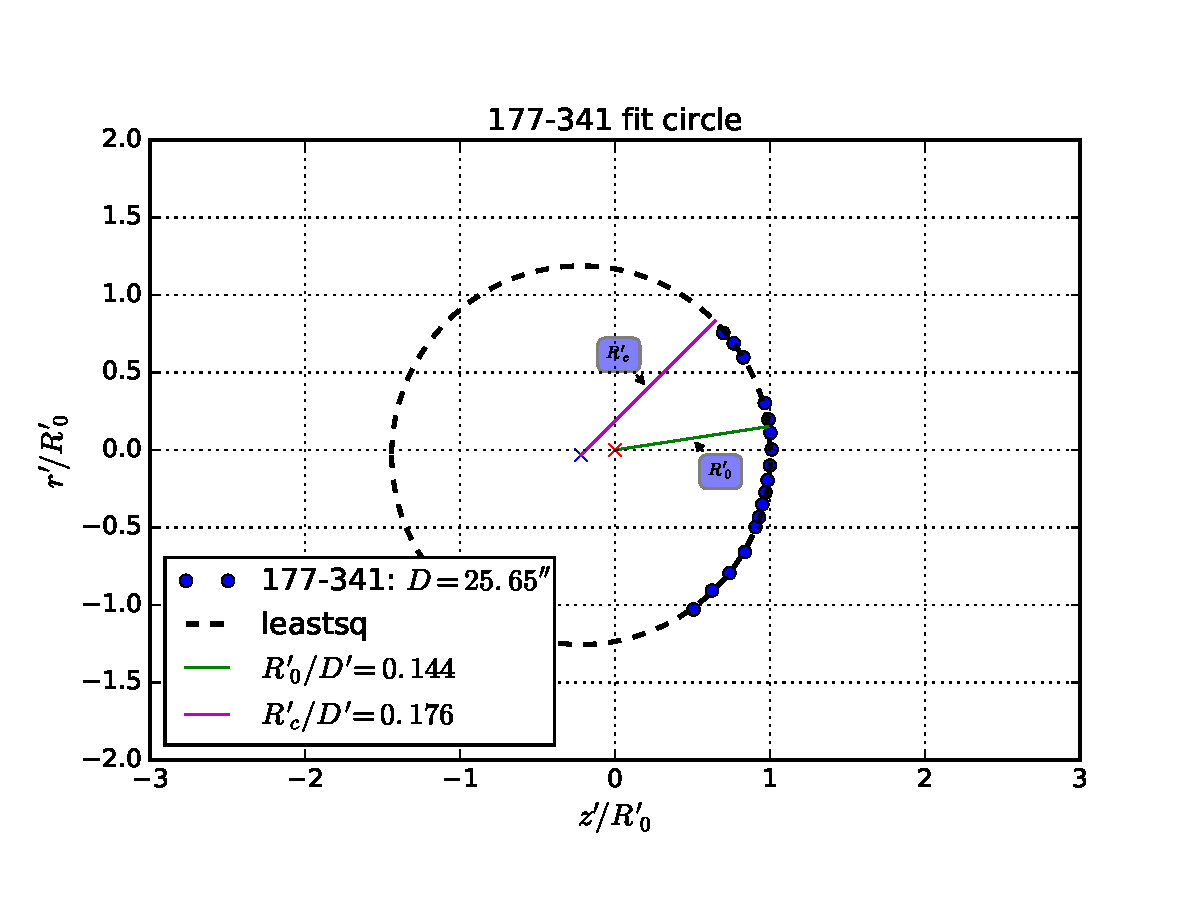
\includegraphics[clip]{../../read-shapes/LV-bowshocks-xyfancy-positionswill-177-341} & 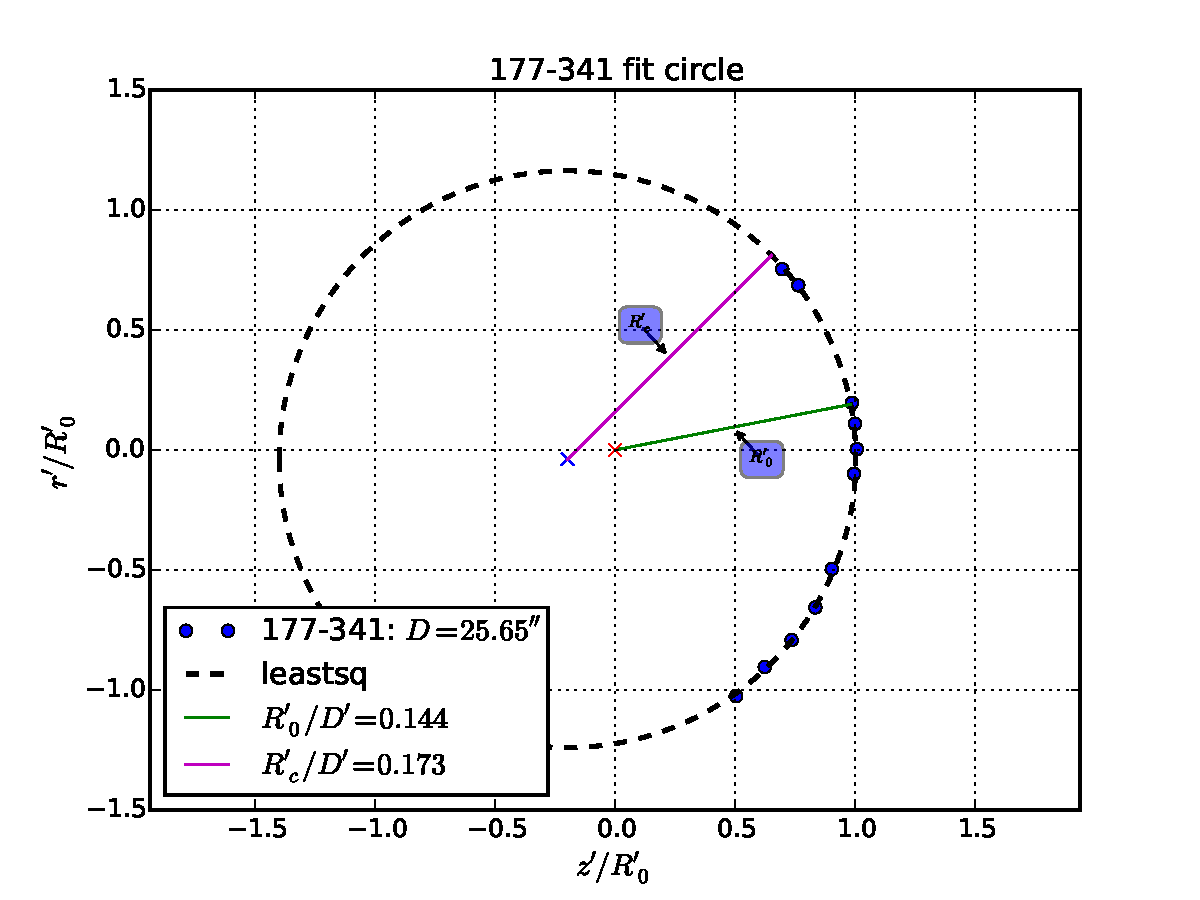
\includegraphics[clip]{../../read-shapes/Multi-Fit/samp00/LV-bowshocks-xyfancy-positionssamp00-177-341} &
  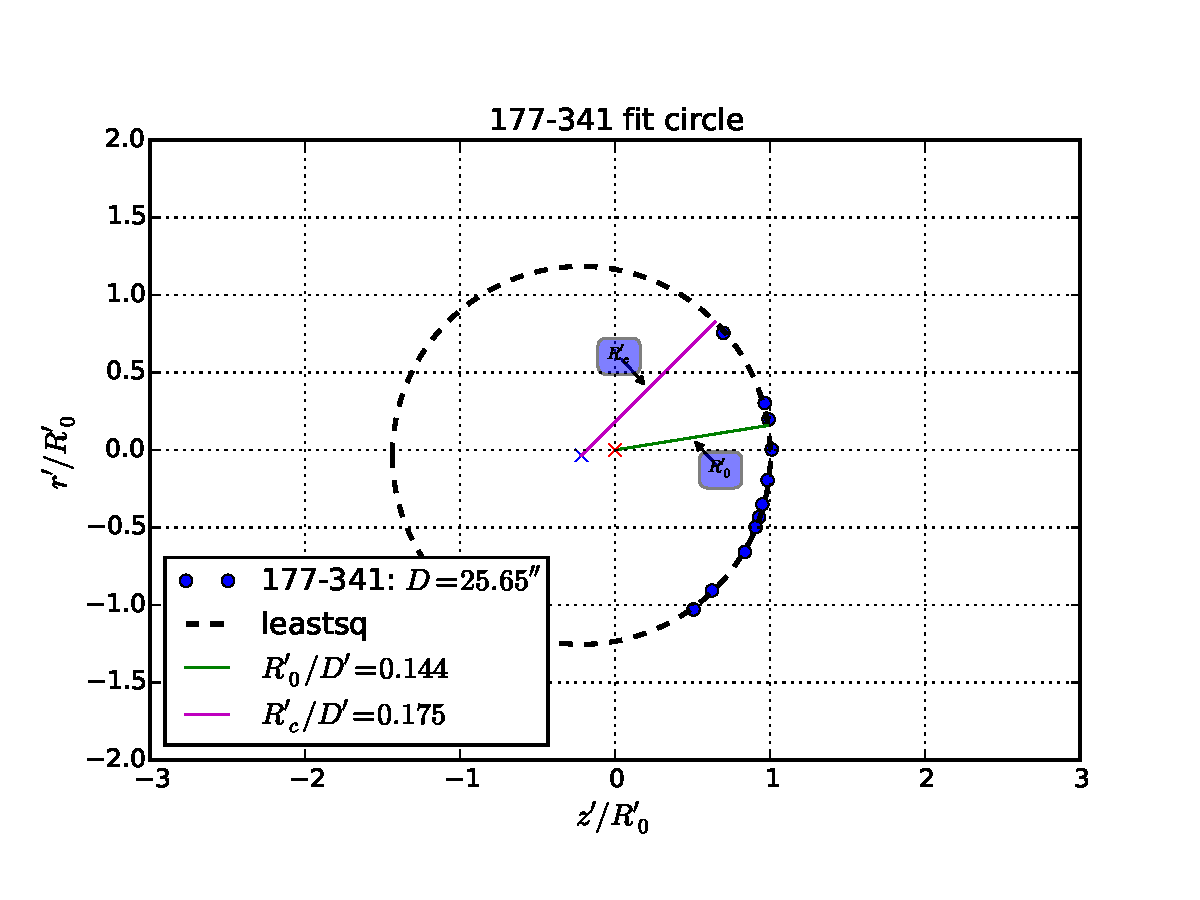
\includegraphics[clip]{../../read-shapes/Multi-Fit/samp01/LV-bowshocks-xyfancy-positionssamp01-177-341} \\
  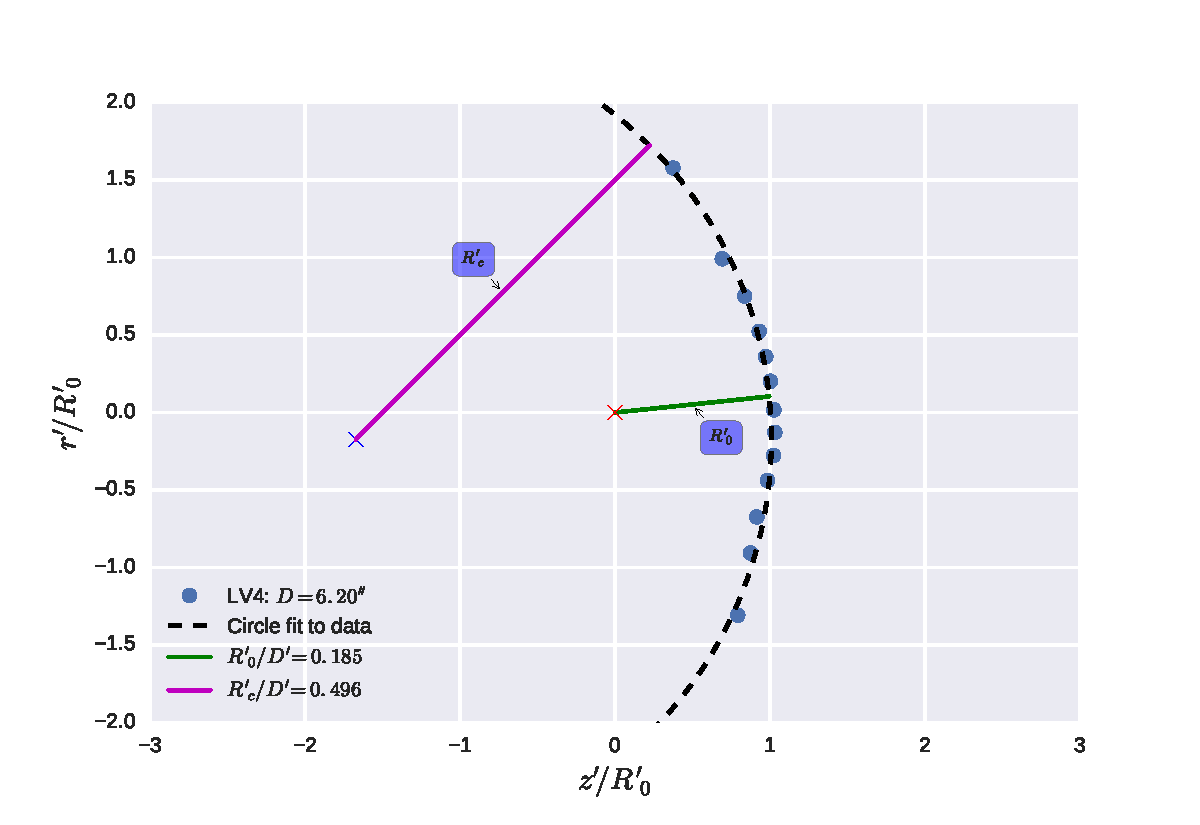
\includegraphics[clip]{../../read-shapes/LV-bowshocks-xyfancy-positionswill-LV4} & 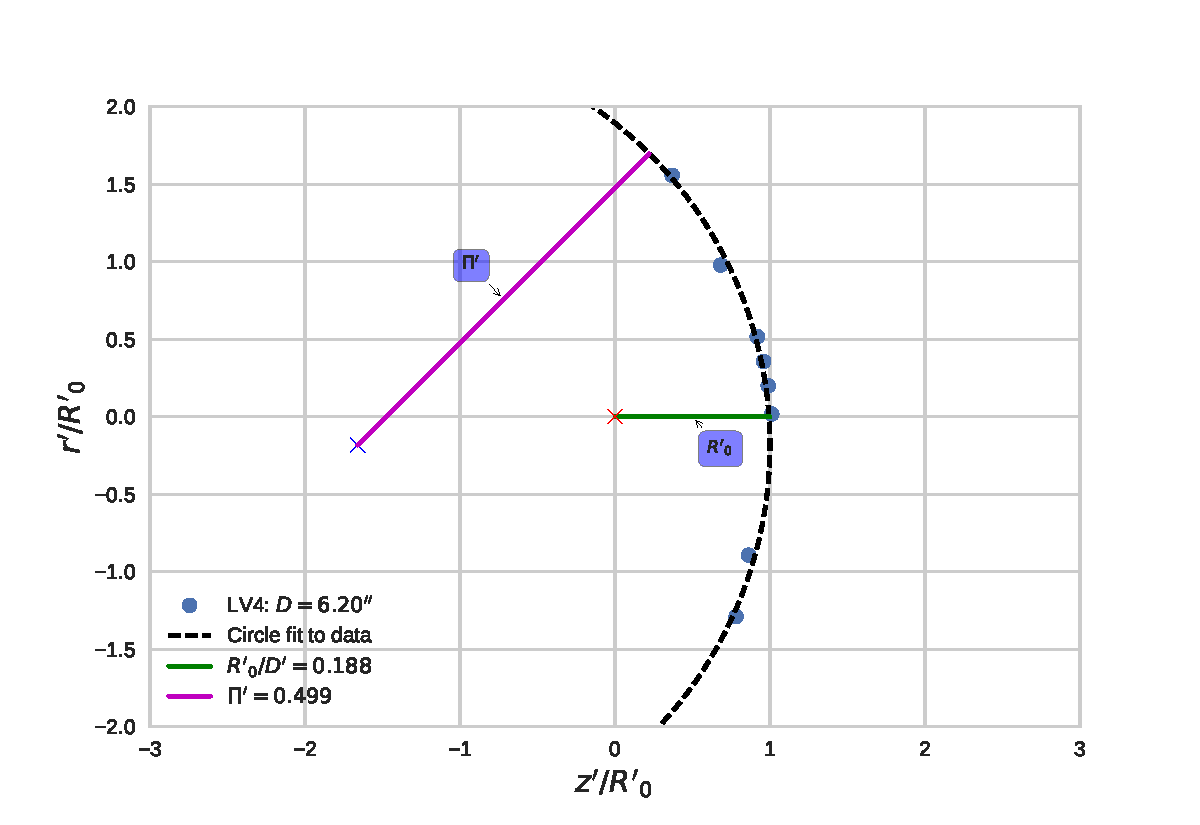
\includegraphics[clip]{../../read-shapes/Multi-Fit/samp05/LV-bowshocks-xyfancy-positionssamp05-LV4} &
  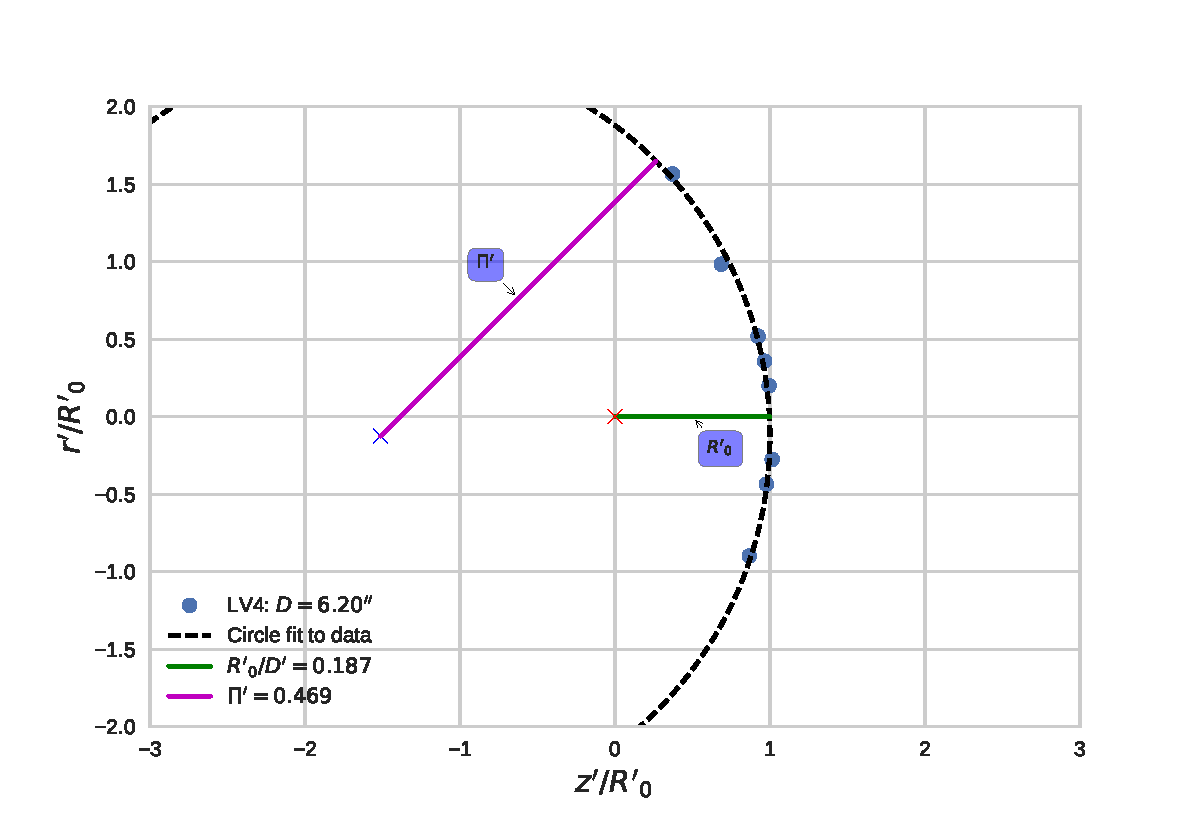
\includegraphics[clip]{../../read-shapes/Multi-Fit/samp01/LV-bowshocks-xyfancy-positionssamp01-LV4} \\
  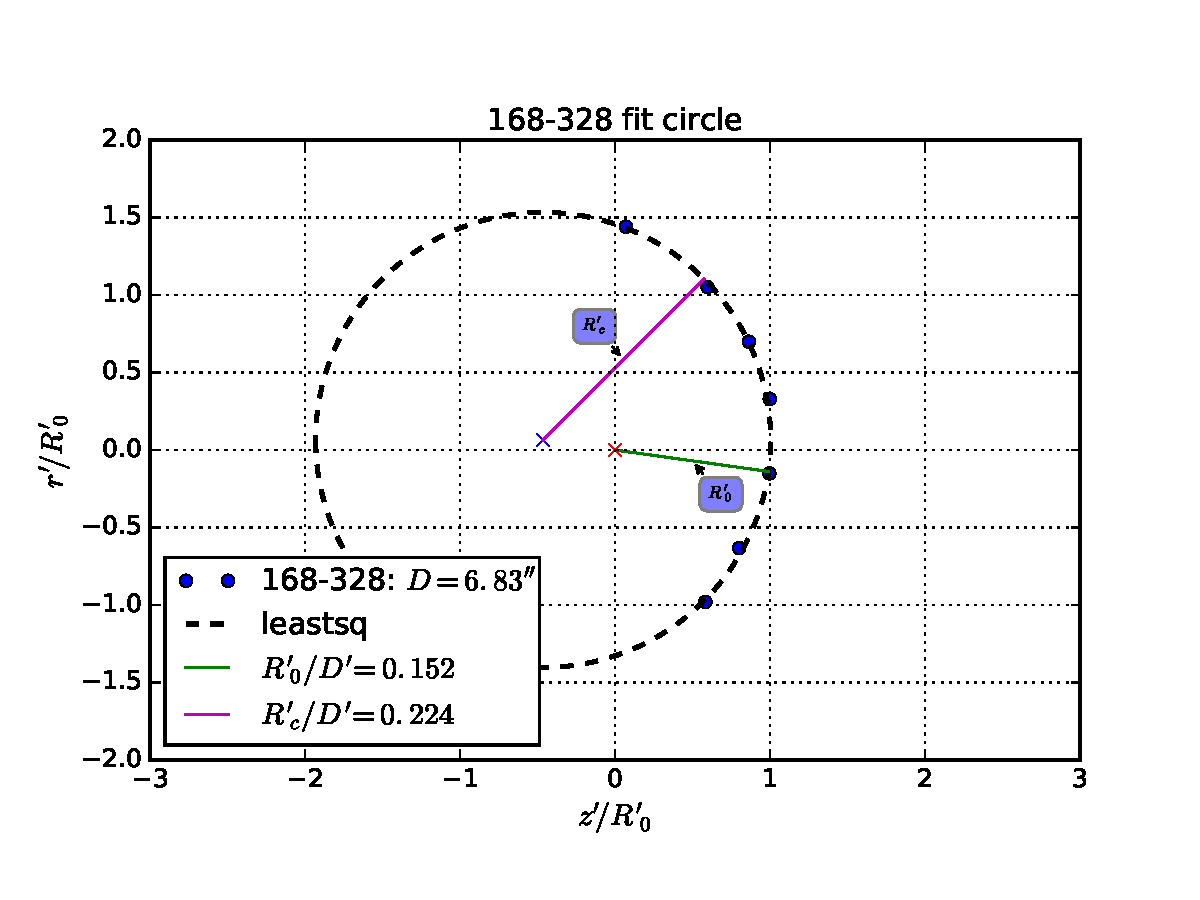
\includegraphics[clip]{../../read-shapes/LV-bowshocks-xyfancy-positionswill-168-328} & 
  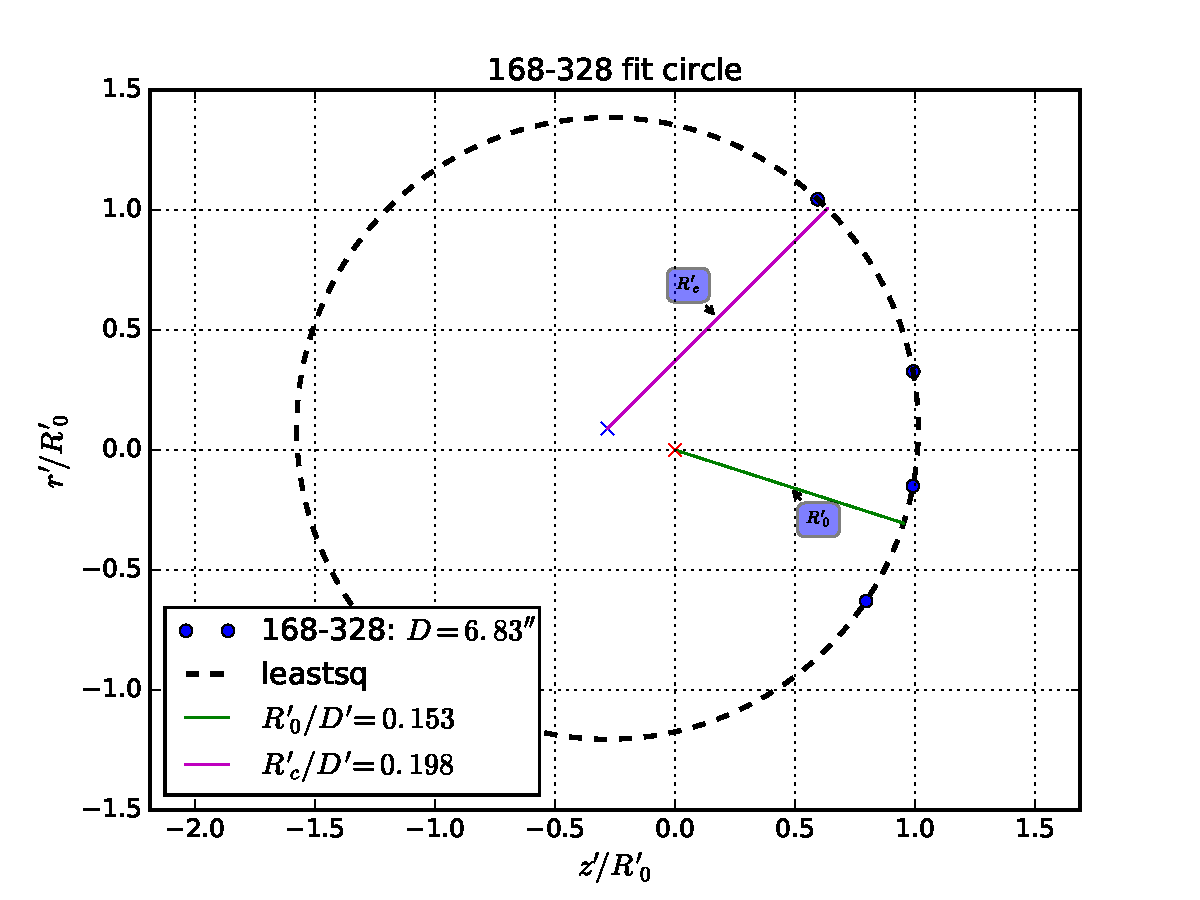
\includegraphics[clip]{../../read-shapes/Multi-Fit/samp00/LV-bowshocks-xyfancy-positionssamp00-168-328} & 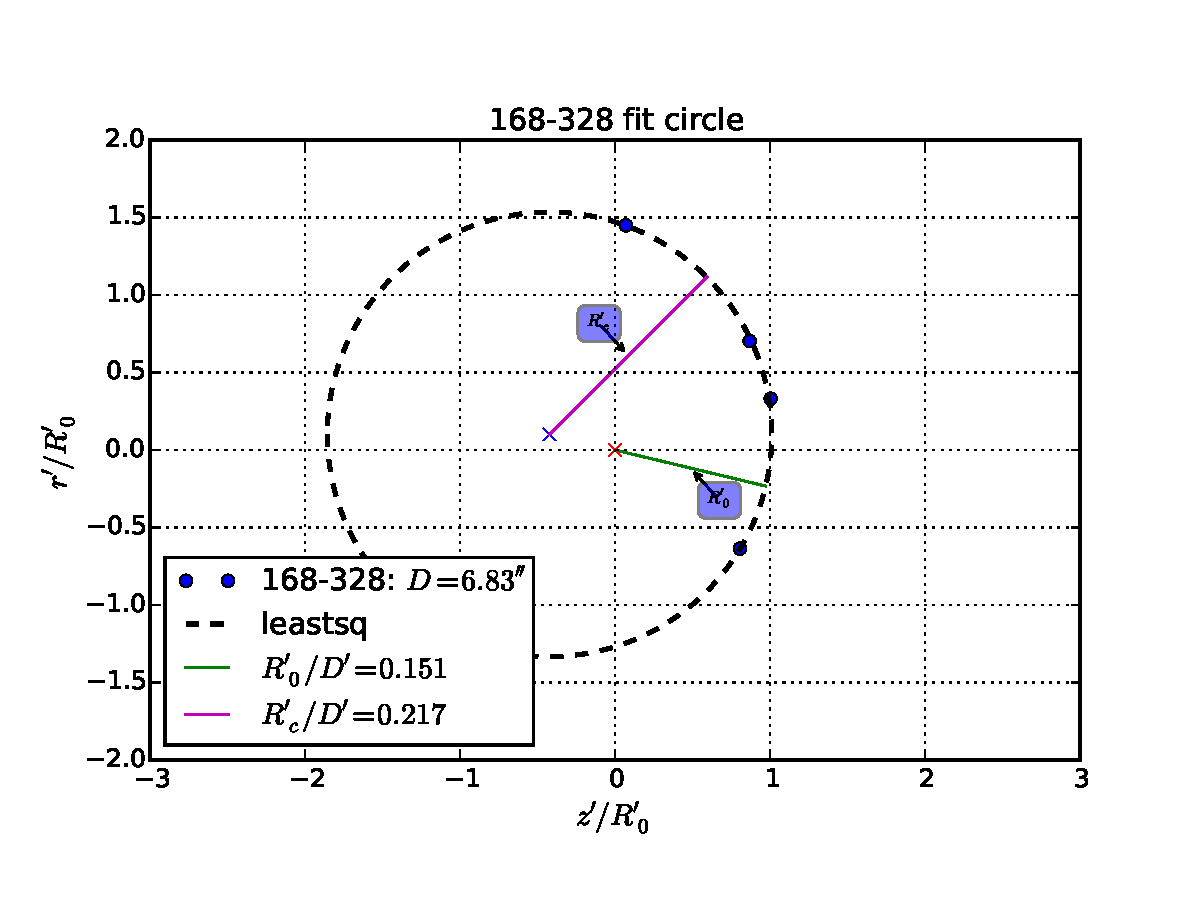
\includegraphics[clip]{../../read-shapes/Multi-Fit/samp01/LV-bowshocks-xyfancy-positionssamp01-168-328}
\end{tabular}
\caption{Examples of systematic uncertainties in the circle fits to
  the shell shapes for three sources (top to bottom rows): 177-341,
  LV4 and 168-328.  The left hand column shows the fit to all of the
  points identified on the shell border, where the number and spacing
  of the points is a subjective measure of our confidence in tracing
  the edge of each shell. The remaining two columns show fits to
  randomly selected sub-samples of 2/3 of the points for each shell.}
\label{fig:char-radii-obs}
\end{figure*}

%\subsection{Conic Scenario}


 

\begin{figure*}
\begin{tabular}{cc}
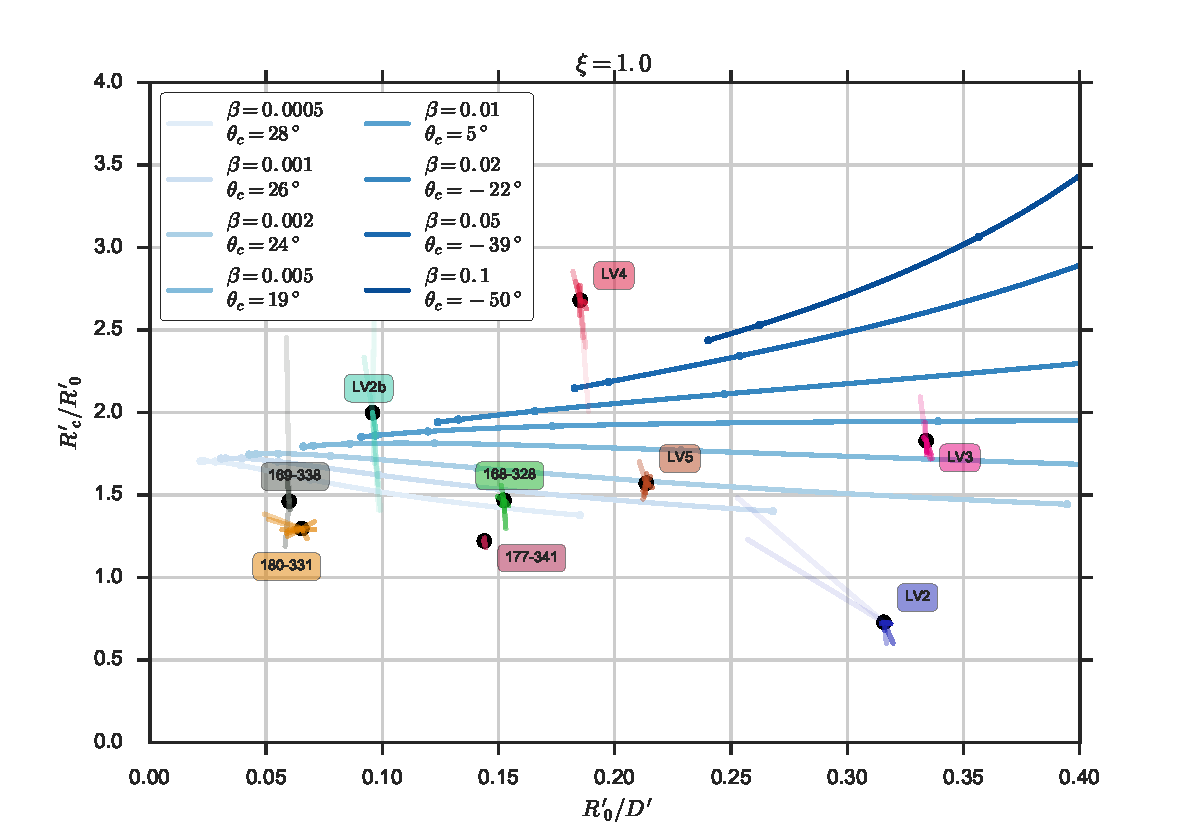
\includegraphics[width=0.48\linewidth]{../../read-shapes/conic_xi-10} & 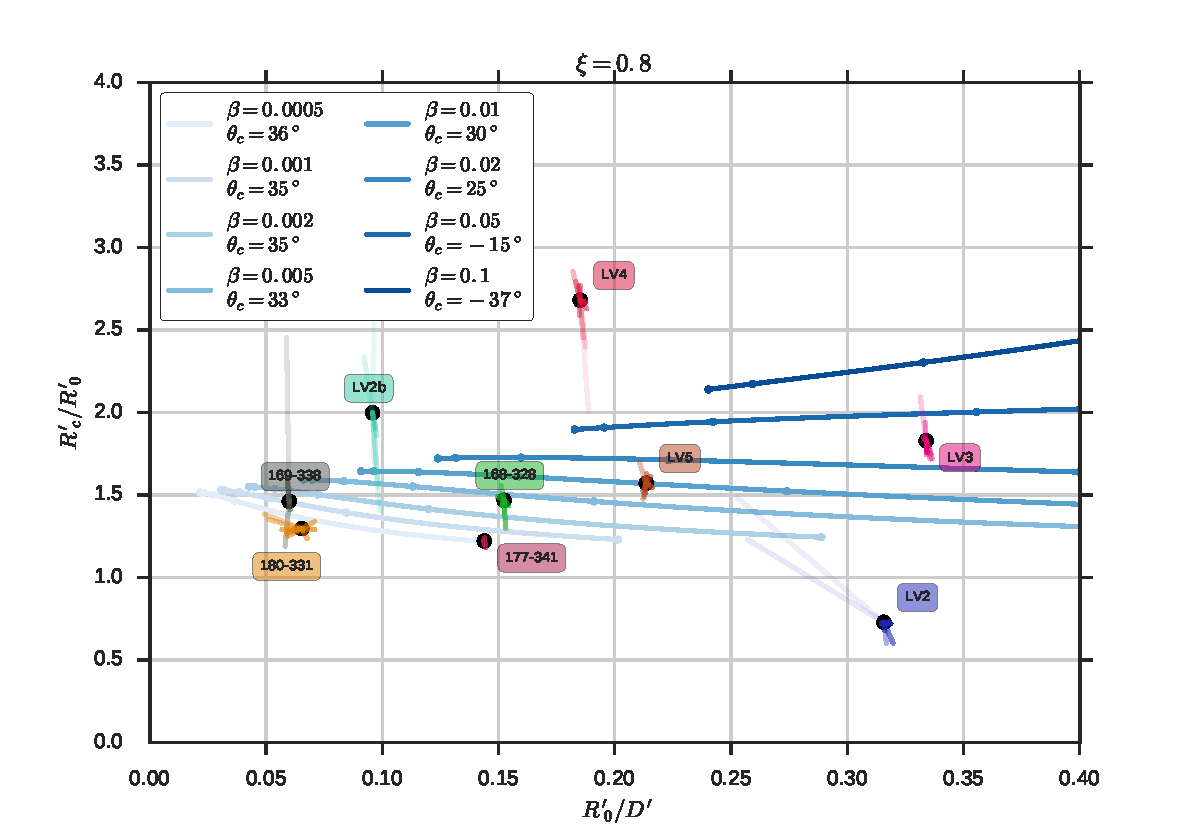
\includegraphics[width=0.48\linewidth]{../../read-shapes/conic_xi-08} \\
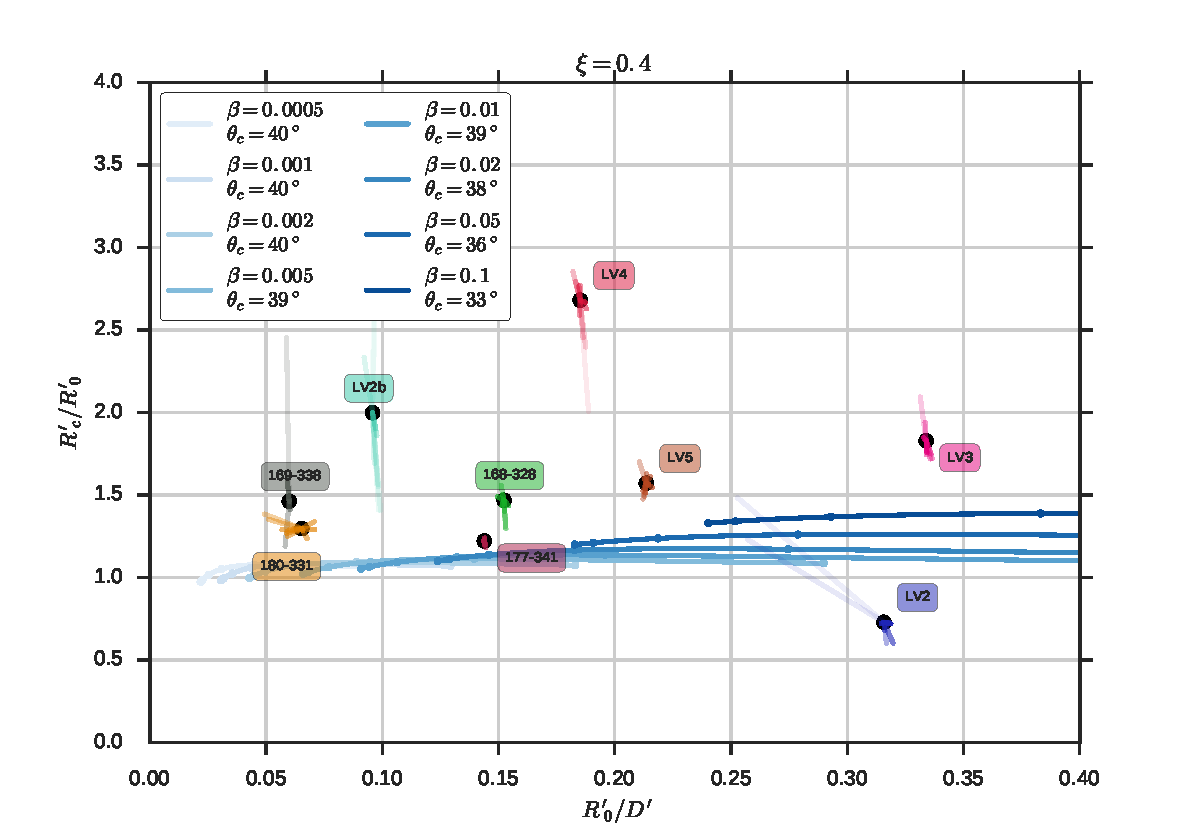
\includegraphics[width=0.48\linewidth]{../../read-shapes/conic_xi-04} & 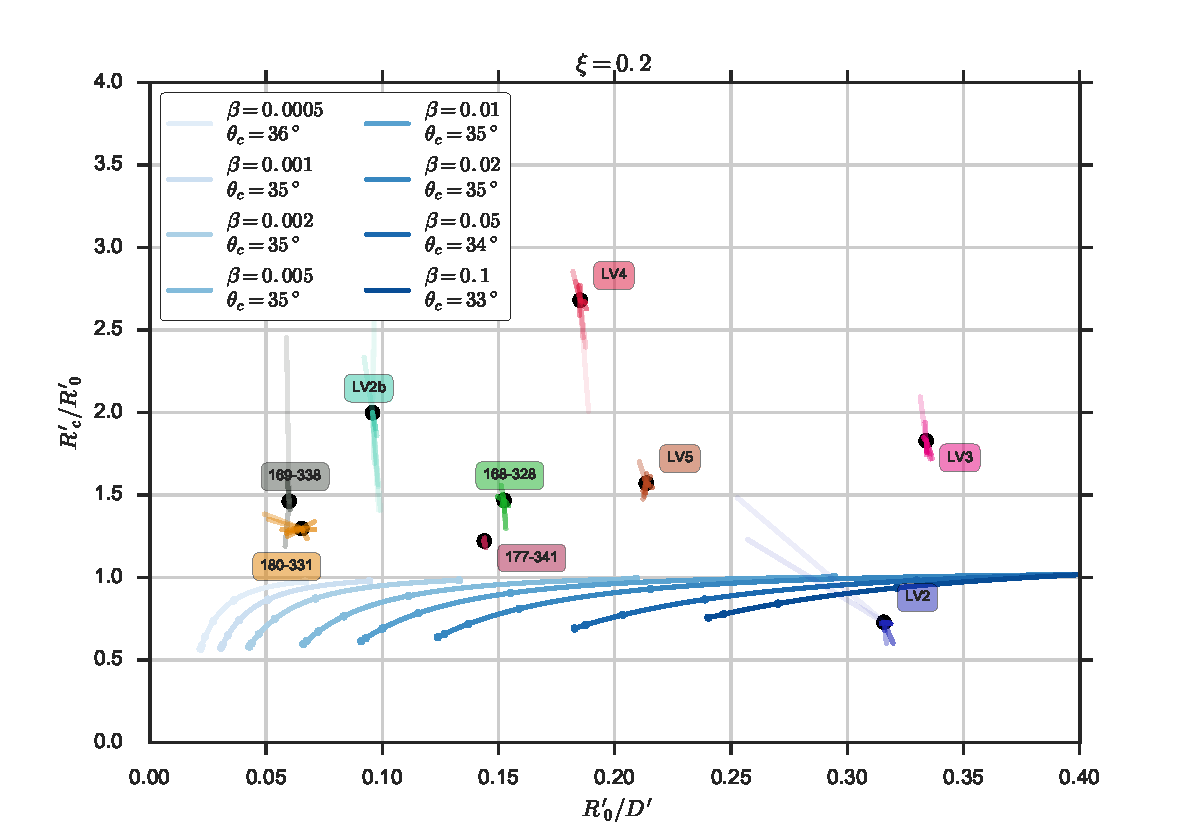
\includegraphics[width=0.48\linewidth]{../../read-shapes/conic_xi-02} 
\end{tabular}
\caption{Measurements of proplyd's characteristic radii $R_c$ and $R_0$. The curves represent a conic-like bow shock with 
fixed momentum ratio $\beta$ and the derived value of $\theta_c$ is also shown.The dots along each curve represent separation in inclination of 
$15^\circ$. The measurements of each proplyd are accompained with the set of variations represented as colored radial lines. In 
each graph we use a different degree of the weaker wind anisotropy, starting from an isotropic wind $(\xi=1)$, to the most anisotropic wind
$(\xi=0.2)$.}
\label{fig:conic-xi}
\end{figure*}

\begin{figure}
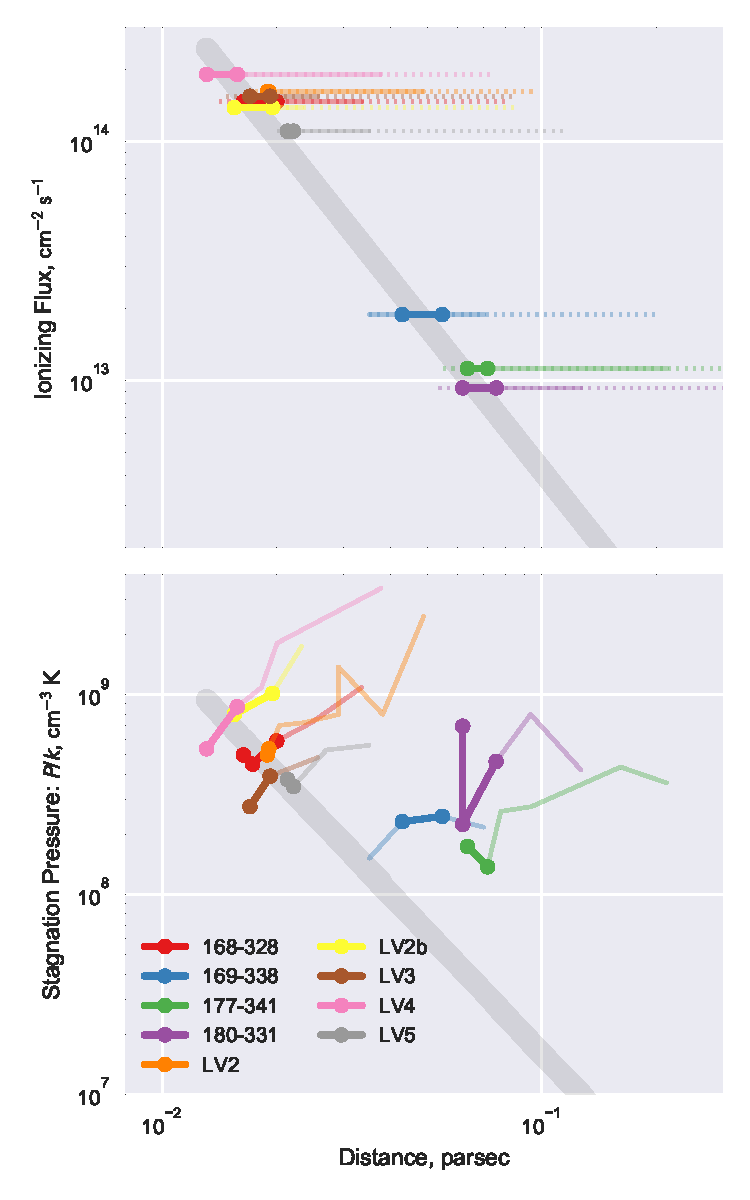
\includegraphics[width=\linewidth]{../../proplyd-wind-figs/plot-wind-fits}
\caption{Top: In colored lines, we show the ionizing flux required to balance the photoevaporated flow for some models which agree with the observed radii for each proplyd compared against the stellar ionizing 
flux at the distance D.
Bottom: The estimated stagnation pressure for the same models as above compared against the stellar wind pressure.
In both graphs, the big dots represent th models which show agreement with ionization balance.}
%\caption{Top: In colored lines,  the required ionizing flux to balance the photoevaporated flow for each proplyd. The gray line represents the stellar flux at the distance $D$. 
%Bottom: In colored lines, estimated stagnation pressure for each proplyd. 
%The gray solid line represent the stellar wind at the distance $D$. in both cases, the big dots represent the variations which have more agreement with ionization balance and pressure balance, respectively.}
\label{fig:pressure}
\end{figure}

\begin{table*}
  \caption{Fitted arc parameters for proplyd bowshocks}
  \label{tab:arc-fits} 
\newcommand\C[1]{\multicolumn{1}{c}{#1}}
\begin{tabular}{llrllllrlll}\toprule
             &          & \multicolumn{3}{c}{\dotfill Observed \dotfill}              & \multicolumn{6}{c}{\dotfill Model fits \dotfill} \\ 
  \C{OW}     & \C{Name} & \(D'\) &\C{ \(R_0'/D'\) }&\C{ \((R_c'/R_0')_{\mathrm{shape}}\) }&\C{ \((R_c'/R_0')_{\mathrm{flux}}\) }&\C{ \(\beta\) }&\C{ \(\xi\) }&\C{ \(|i|\) }&\C{ \(D\) }&\C{ \(R_0/D\)}\\
  \C{(1)}& \C{ (2) }&\C{ (3)    }&\C{    (4)      }&\C{              (5)           }&\C{           (6)             }&\C{     (7)   }&\C{   (8)   }&\C{   (9) }&\C{  (10) }&\C{   (11)} \\
\midrule     
 168-328  &            &    6.8  &  $0.152 \pm 0.001$  &  $1.42 \pm 0.09$   &  $1.45 \pm 0.05$     &  $0.018 \pm 0.003$  &  0.4 -- 0.6  &  $33 \pm 3$   &  $0.017 \pm 0.001$  &  $0.115 \pm 0.005$  \\
 169-338  &            &  16.4  &  $0.059 \pm 0.001$  &  $1.76 \pm 0.48$   &  $1.50 \pm 0.05$     &  $0.002 \pm 0.001$  &  0.8 -- 0.8  &  $43 \pm 8$   &  $0.049 \pm 0.006$  &  $0.035 \pm 0.005$  \\
 177-341  & HST1   & 25.6  &  $0.144 \pm 0.001$  &  $1.21 \pm 0.02$   &  $1.25 \pm 0.02$     &  $0.018 \pm 0.003$  &  0.1 -- 0.2  &  $30 \pm 5$   &  $0.064 \pm 0.003$  &  $0.115 \pm 0.005$  \\
 180-331  &             &  25.1  &  $0.061 \pm 0.007$  &  $1.30 \pm 0.05$   &  $1.27 \pm 0.05$     &  $0.003 \pm 0.001$  &  0.4 -- 0.4  &  $35 \pm 7$   &  $0.066 \pm 0.007$  &  $0.047 \pm 0.005$  \\
 167-317  &  LV2     &    7.8  &  $0.305 \pm 0.025$  &  $0.81 \pm 0.28$   &  $1.50 \pm 0.1$      &  $0.085 \pm 0.015$  &  0.1 -- 0.2  &  $13 \pm 13$  &  $0.017 \pm 0.001$  &  $0.225 \pm 0.005$  \\
               & LV2b    &   7.2  &  $0.097 \pm 0.002$  &  $2.00 \pm 0.62$   &  $1.63 \pm 0.08$     &  $0.008 \pm 0.003$  &  0.8 -- 0.8  &  $28 \pm 13$  &  $0.018 \pm 0.002$  &  $0.078 \pm 0.013$  \\
 163-317  & LV3      &   6.9  &  $0.334 \pm 0.002$  &  $1.81 \pm 0.12$   &  $1.85 \pm 0.15$     &  $0.075 \pm 0.025$  &  0.6 -- 0.8  &  $35 \pm 5$   &  $0.018 \pm 0.001$  &  $0.205 \pm 0.025$  \\
 161-324  & LV4      &   6.2  &  $0.186 \pm 0.002$  &  $2.59 \pm 0.24$   &  $2.05 \pm 0.07$     &  $0.040 \pm 0.014$  &  0.8 -- 1.0  &  $18 \pm 12$  &  $0.014 \pm 0.001$  &  $0.160 \pm 0.028$  \\
 168-323  & LV5      &   9.6  &  $0.213 \pm 0.002$  &  $1.57 \pm 0.07$   &  $1.60 \pm 0.07$     &  $0.055 \pm 0.005$  &  0.2 -- 0.4  &  $20 \pm 5$   &  $0.022 \pm 0.001$  &  $0.190 \pm 0.010$  \\
\bottomrule
\end{tabular}
\begin{minipage}{0.95\linewidth}
  Notes --
%
  Col.~(1): Source ID \citep{ODell:1994a}.
%
  Col.~(2): Alternative name of source.
% 
  Col.~(3): Projected distance from \thC{}, arcseconds.
%
  Col.~(4): Apparent shell outer radius along axis, normalized to
  projected distance, with \(\pm 1\sigma\) uncertainties, determined
  from circle fits described in \S~\ref{sec:methodology}.
% 
  Col.~(5): Apparent shell radius of curvature, normalized to radius
  along axis, with \(\pm 1\sigma\) uncertainties, determined from
  circle fits described in \S~\ref{sec:methodology}.
% 
  Col.~(6): As Col.~(5) but applying the additional requirement that
  the proplyd surface brightness from model fits should agree with the
  theoretical prediction.
%
  Col.~(7): Proplyd-to-O~star wind momentum ratio (see \S~\ref{sec:crw-scenario}). 
% 
  Col.~(8): Proplyd wind anisotropy factor.
% 
  Col.~(9): Inclination to plane of sky, degrees.
% 
  Col.~(10): True distance from \thC{}, parsecs.
%
  Col.~(11): True shell radius along axis, normalized to distance.

\end{minipage}
\end{table*}
%Measurements of proplyd's characteristic radii $R_c$ and $R_0$. The curves represent a single bow shock with fixed wind's momentum ratio $\beta$. 
%The dots represent separations in inclination of $15^{\circ}$. The semitransparent curves represent bow shocks which the inner wind is isotropic and the full colored 
%curves bow shocks which inner wind density decays as $\cos^{1/2}\theta$. The observational measurements are accompained with radial bars which represents the variations 
%with a fraction of the shell's marks removed. Proplyds with less data marks or high asymmetry show higher deviations in the measurements.

% \begin{table*}
\begin{tabular}{c|ccccccccc}\hline
Proplyd & LV2 & LV2b & LV3 & LV4  & LV5 & 177-341 & 168-328 & 169-338 & 180-331\\\hline
$D (\arcsec)$ &7.76 & 7.21 &6.89 & 6.2 & 9.55 & 25.65 & 6.83 & 16.43 & 25.07 \\
$R_c/D$  & 0.23  & 0.19& 0.61  & 0.5  & 0.34  & 0.18  & 0.22 & 0.09 & 0.09\\
$R_0/D$  & 0.32 & 0.1 & 0.34 & 0.19 & 0.21 & 0.14 & 0.15 & 0.06 & 0.07\\
$R_c/R_0$ & 0.73 & 2.00 & 1.83 & 2.68  & 1.57 & 1.22 & 1.47 & 1.46 & 1.30  
\end{tabular}
\caption{Characteristic Radii measurements for a sample of proplyds. %Enhance description when more rows were included
} 

\label{tab:proplyds}
\end{table*}

%%% Local Variables:
%%% mode: latex
%%% TeX-master: "proplyd-bowshocks.tex"
%%% End:


%\begin{figure}
%\end{figure} 

%\begin{figure*}
%\begin{tabular}{cc}
%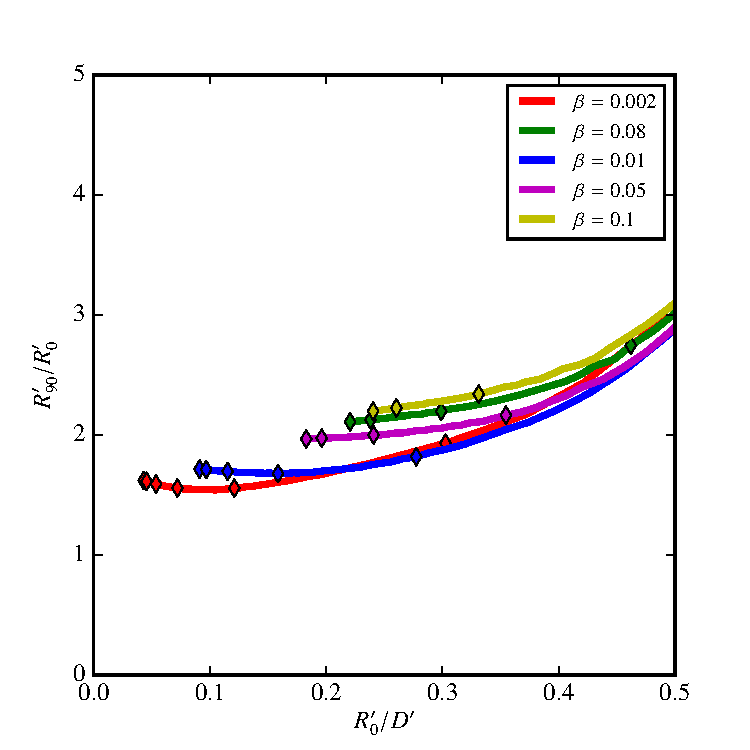
\includegraphics[width=0.5\linewidth]{R90-R0-b}&
%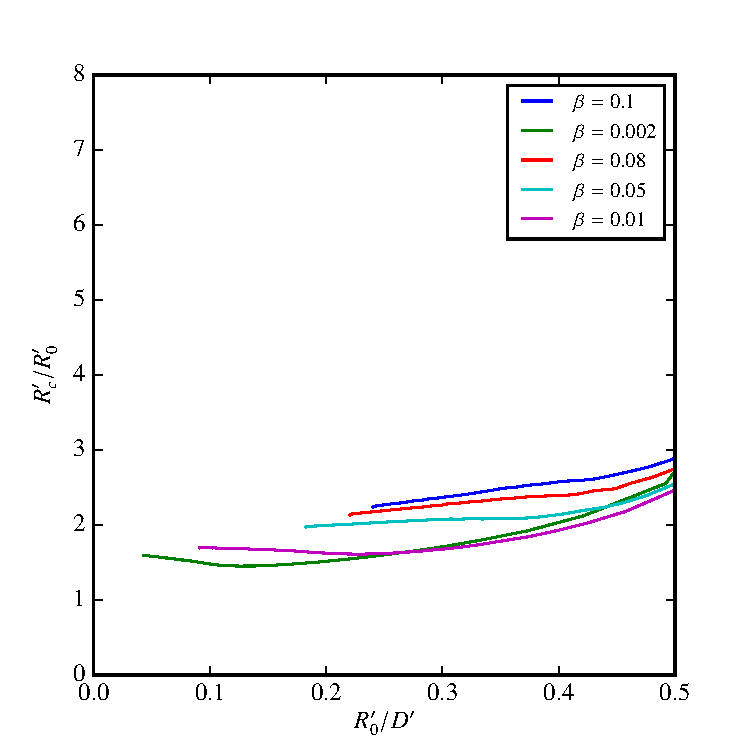
\includegraphics[width=0.5\linewidth]{Rc-R0-b}
%\end{tabular}
%\label{fig:radii-r0}
%\caption{Left: $R_c$ normalized with $R_0$ vs $R_0$ normalized with $D$. Right:$R_{90}$ normalized with $R_0$ vs $R_0$ normalized with $D$. Since the bow shock brightness decays 
%at the wings, it is more difficult to measure $R_{90}$. Along every single curve, $\beta$ is constant. The marks in the curves represents jumps of $15^\circ$ in inclination, and the most left 
%mark in each curve represent $i=0^\circ$}
%\end{figure*}

%is $(0,0)$ and measured distances in arcseconds. In this reference, the proplyd-$\theta_1^C$ line is $y=0$. With the shell's positions, we optimize a circle, whose radius is $R_c$, but
%this optimization has two variants: the first one with the restriction that the center of the circle must lie in the symmetry axis (y=0), and the second variation is with no restrictions. $R_0$ is calculated as the distance between the proplyd position and the bow shock in a line which is also included the
%center of curvature. The figure (\ref{fig:radii-measures-example}) shows a representation of the metodology described. 
%Our first goal was comparing measurements of $(R_0,R_{90})$ of the LV group of proplyds in mid infrared by \citep{Robberto:2005} against observations in [OIII] with better angular resolution but less contrast against
%the background.
%In \citep{Robberto:2005} they compare their observations with shells obtained with the \citep{Canto:1996} two winds interactions formalism. They found no concordance between the model and observations. We attempted to redo the measurements with better resolution observations. We found quickly that we cannot measure $R_{90}$ in a reliable way since the shell's brightness decays toward the wings. Also, we are using a more sophisticated model where the proplyd's wind density decays as $n \propto \cos {1/2}\theta$ instead of an isotropic wind.
%A better replacement of $R_{90}$ is the radius of curvature, defined as the radius of the circle that fits the observations, because always is measurable. Figures (\ref{fig:char-radii-obs}) and (\ref{fig:char-radii-obs-2}) show our measurements of the radius of curvature for the LV group, with exception of LV1, which actually is a binary proplyd, thus our model is not adequate in this case. Also we include the proplyds 167-328, 169-338, 177-341 (HST1), 189-339 and 180-331 which are close enough to $\theta^1~\mathrm{C~Ori}$ to be influenced by it stellar wind.
%Our results show a better concordance (but still not perfect) between models and observations, as shown in figure (\ref{fig:prop-shell-err}). A possible cause of the discrepancy may be that the \citep{Canto:1996} model assumes that the interacting winds are hypersonic in such way that the shocked gas can be considered as a bidimensional surface. In practice, the bow shock has a finite width, which can afect the apparent shape due to projection effects

%Initially we tried to measure the radii $(R_0,R_{90})$, but it wasn't possible due to the fact that the brightness of the shell decays rapidly towards the wings, and using $R_\theta$ where $60 \lesssim \theta < 0 $ is not so useful, because there is not a significant difference between $R_0$ and $R_\theta$. Instead, we introduced the radius of curvature after we realized how well the shell's marks fits into a circle for all the proplyds (see figure (\ref{fig:char-radii-obs})).

%\begin{figure*}
%\begin{tabular}{cc}
%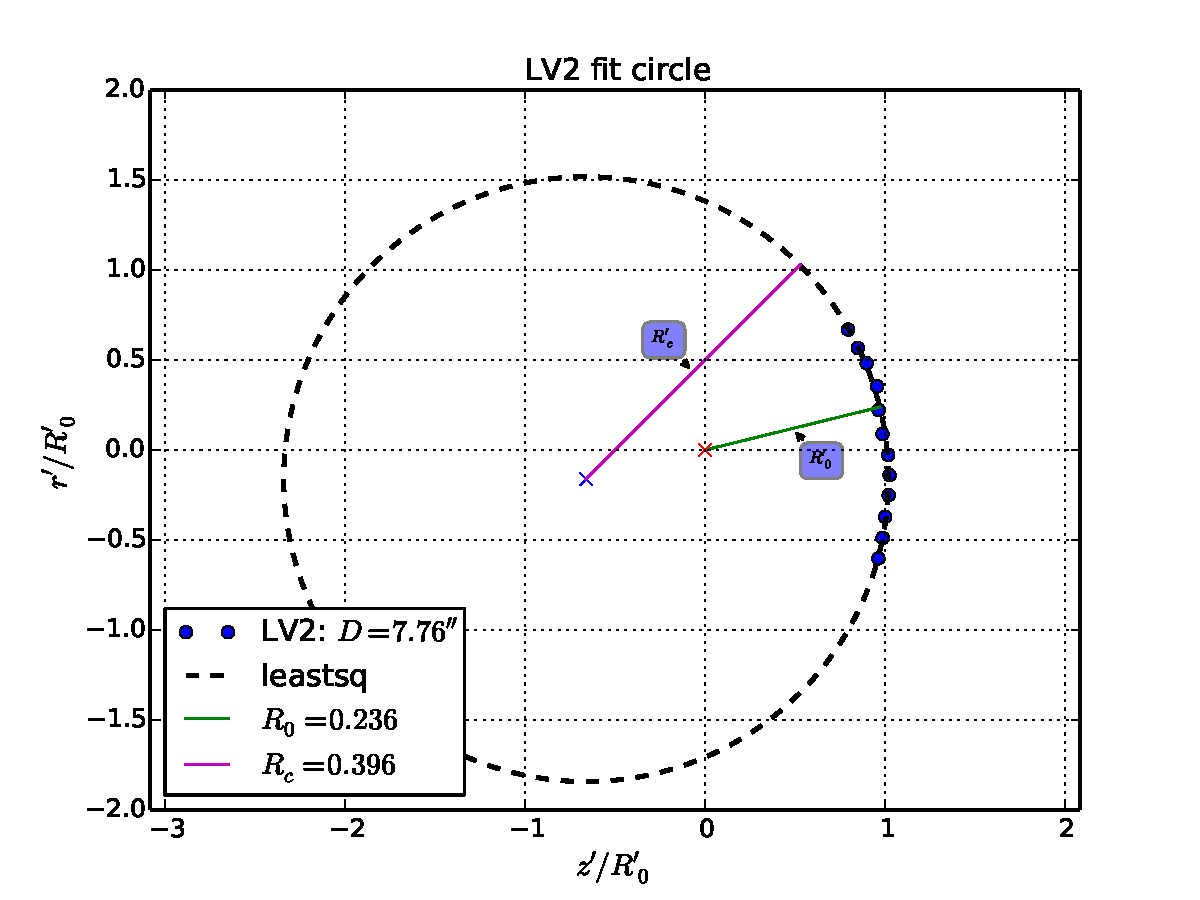
\includegraphics[width=0.5\linewidth]{LV-bowshocks-xyfancy-502epositions-LV2} & 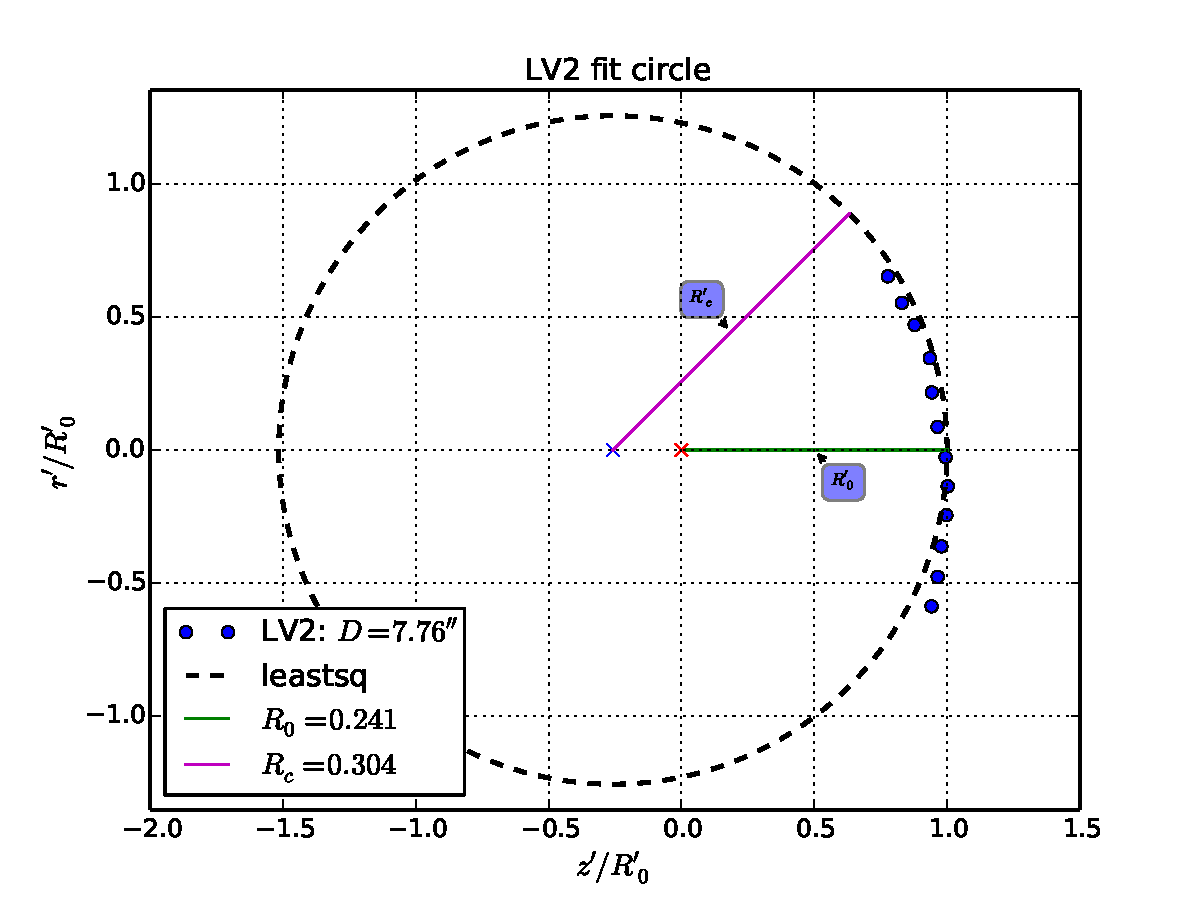
\includegraphics[width=0.5\linewidth]{LV-bowshocks-xyfancy-onaxis-502epositions-LV2} \\
%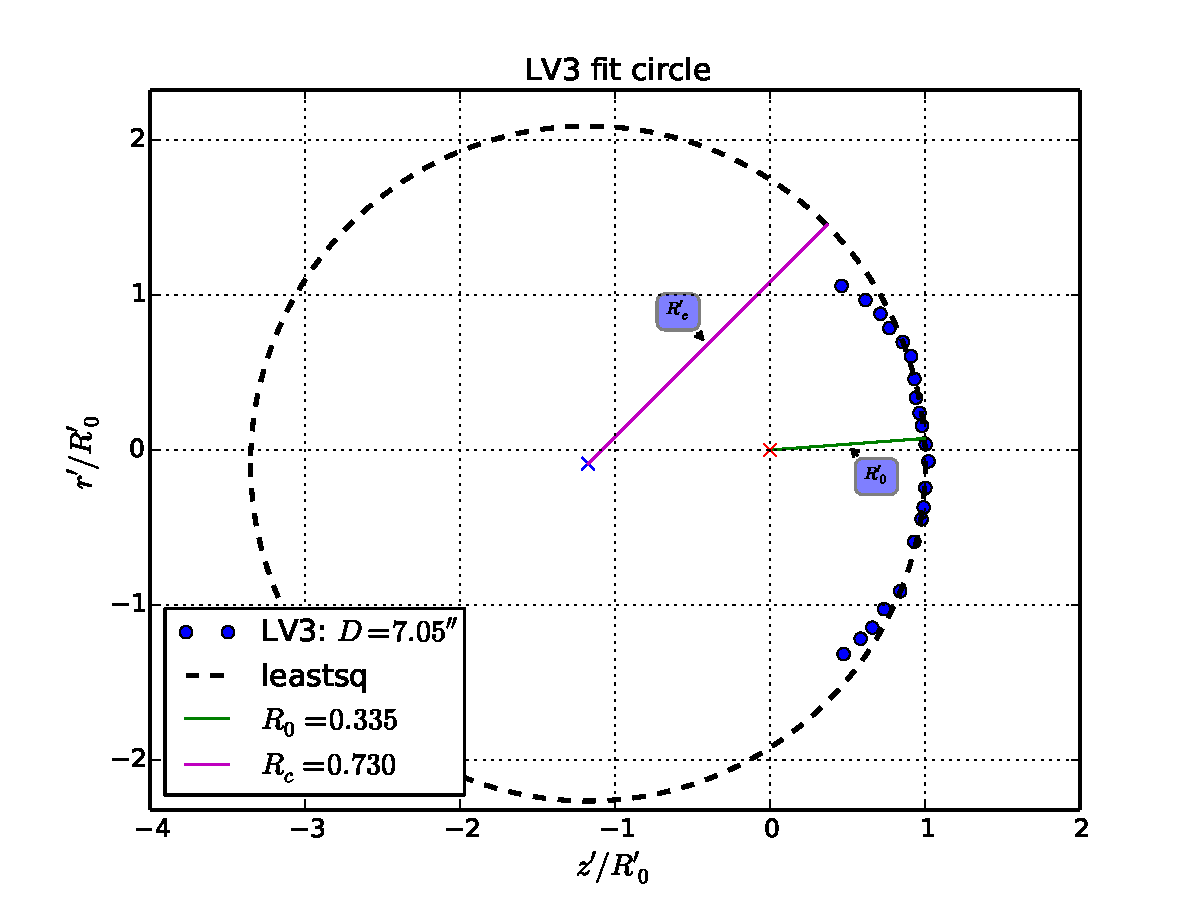
\includegraphics[width=0.5\linewidth]{LV-bowshocks-xyfancy-OIII3a-LV3} & 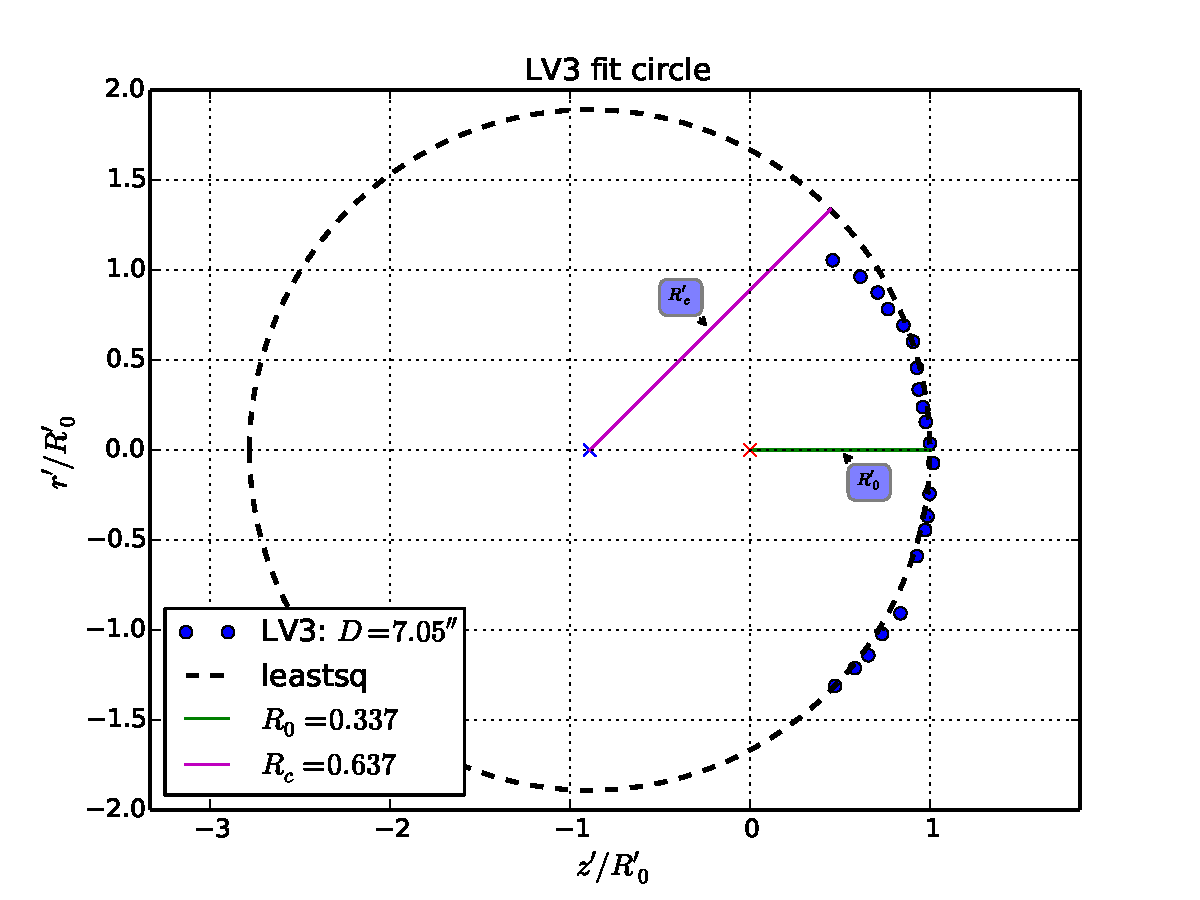
\includegraphics[width=0.5\linewidth]{LV-bowshocks-xyfancy-onaxis-OIII3a-LV3} \\
%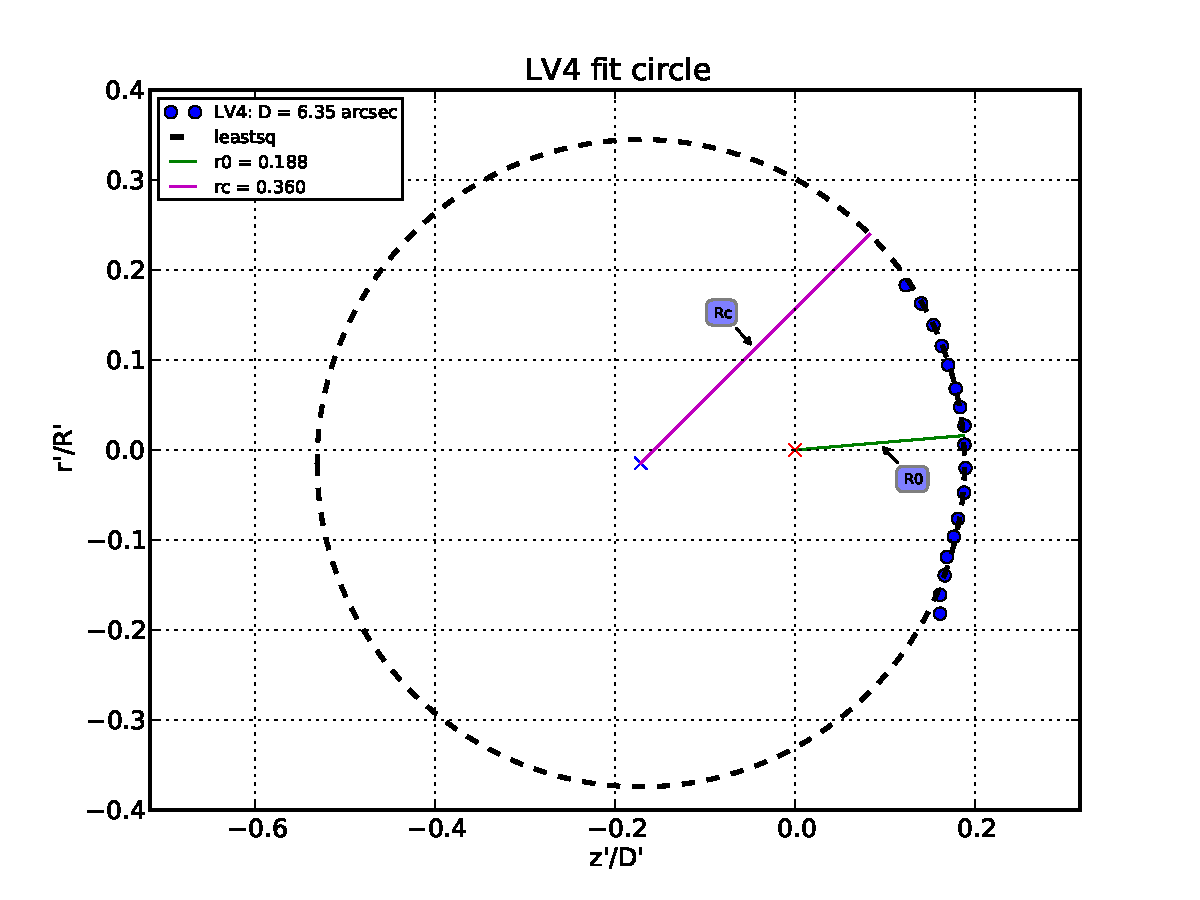
\includegraphics[width=0.5\linewidth]{LV-bowshocks-xyfancy-OIII3a-LV4} & 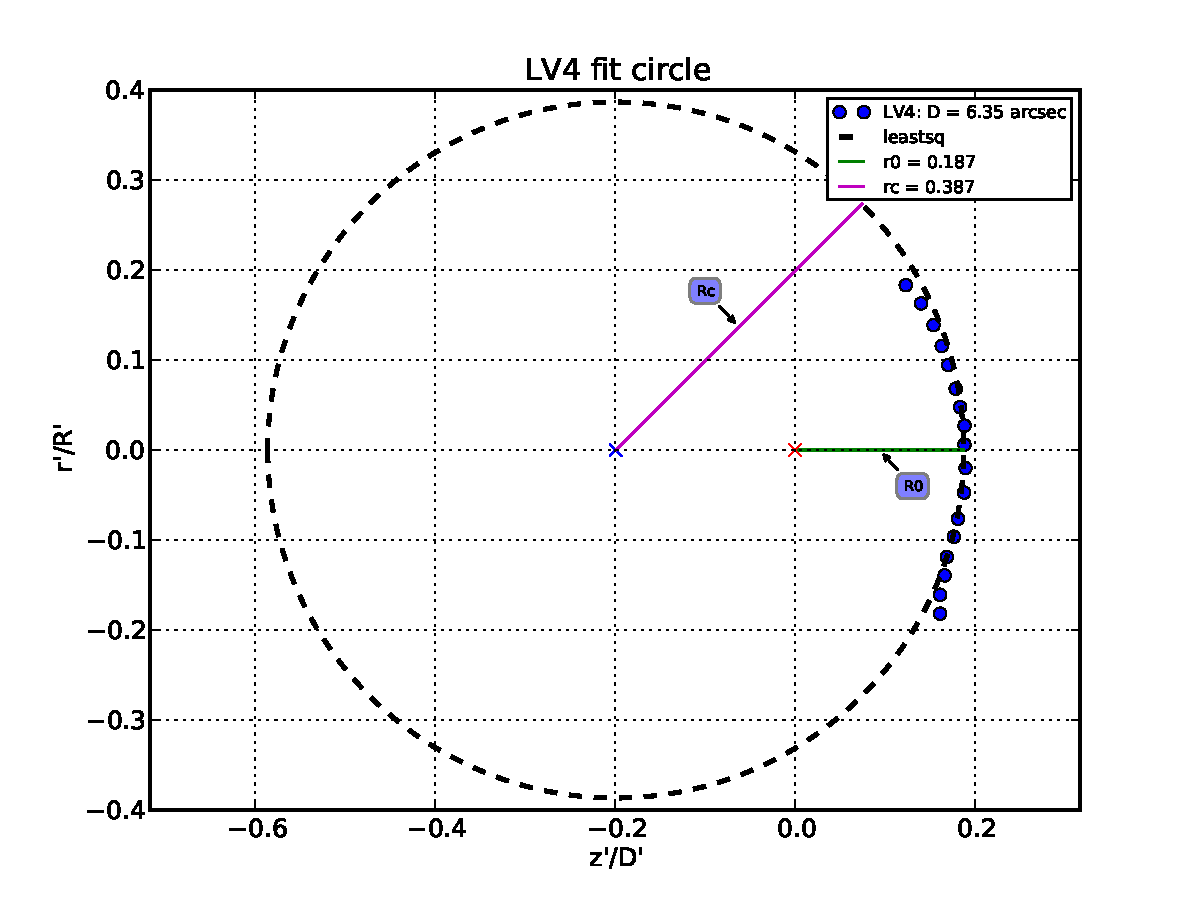
\includegraphics[width=0.5\linewidth]{LV-bowshocks-xyfancy-onaxis-OIII3a-LV4}
%\end{tabular}
%\label{fig:char-radii-obs}
%\caption{Fits to the shell's shapes. In the left side we have the fits without any restrictions. In the right side we have the fits restricting the center of the circle to be in $y=0$. This data is summarized in table (\ref{tab:proplyds})}
%\end{figure*}

%\begin{figure*}
%\begin{tabular}{cc}
%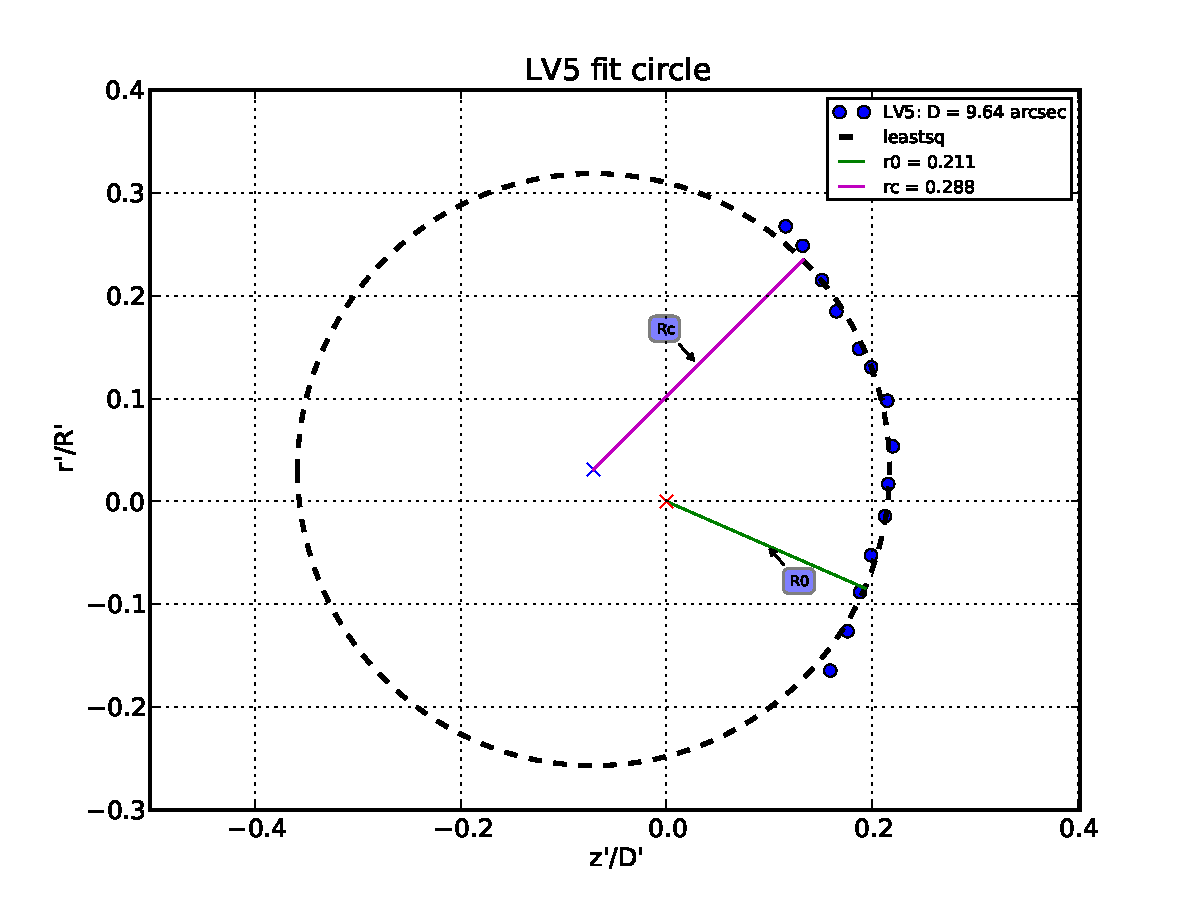
\includegraphics[width=0.5\linewidth]{LV-bowshocks-xyfancy-OIII3a-LV5} & 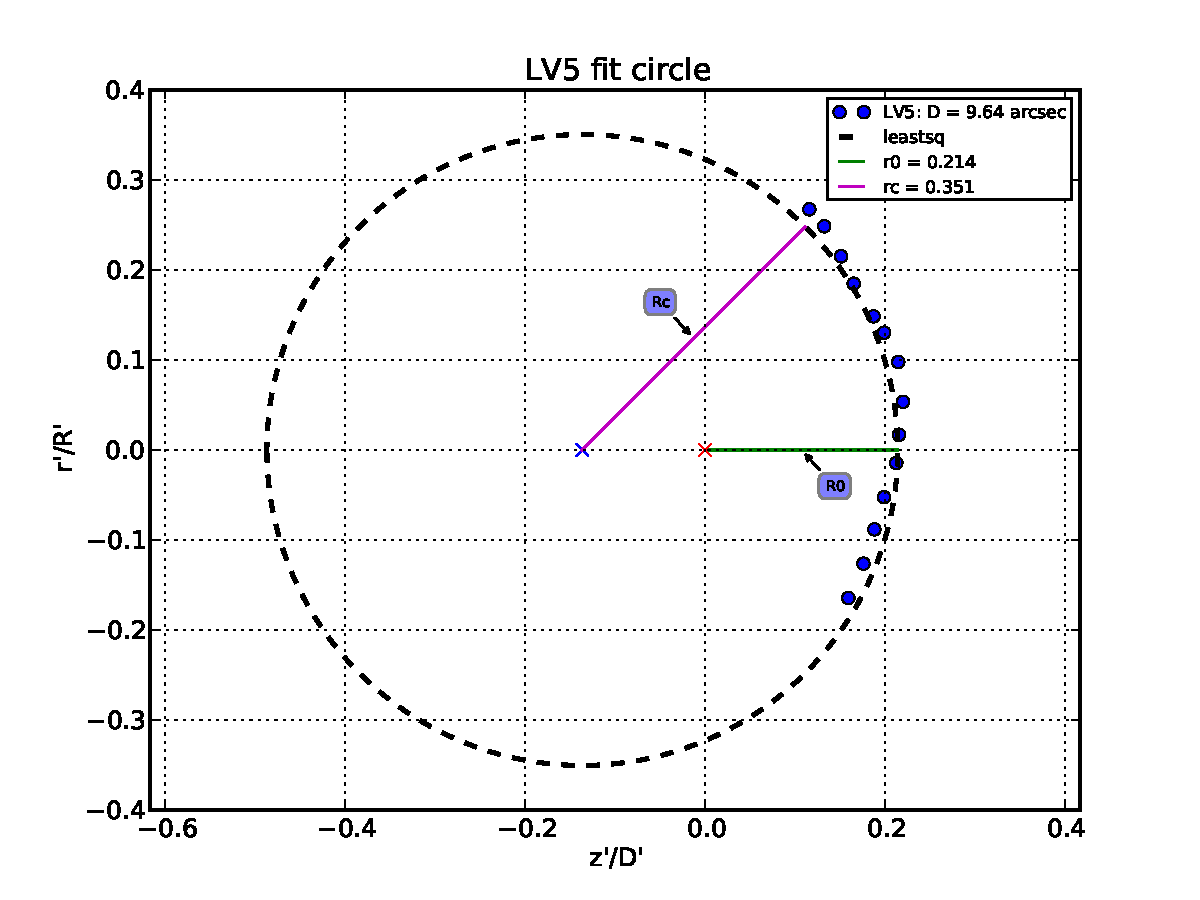
\includegraphics[width=0.5\linewidth]{LV-bowshocks-xyfancy-onaxis-OIII3a-LV5} \\
%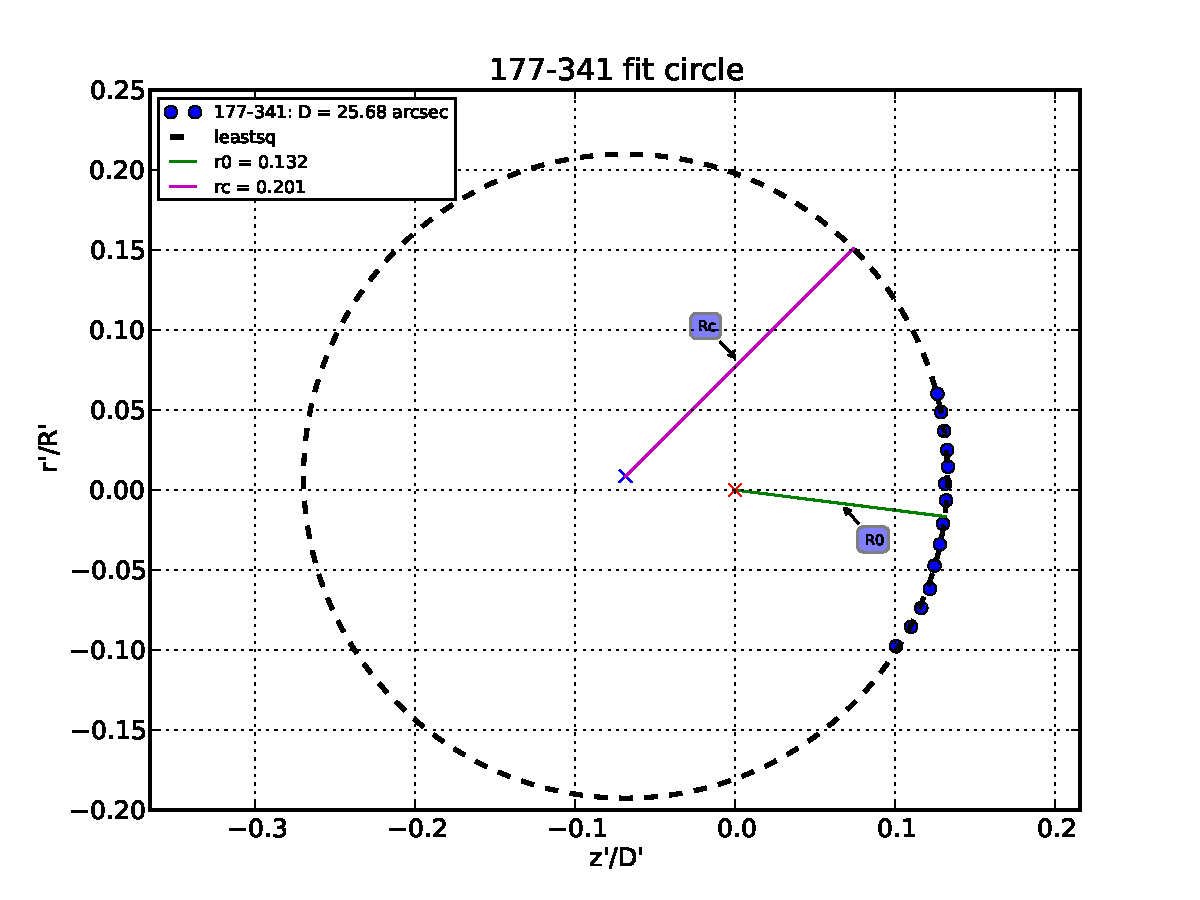
\includegraphics[width=0.5\linewidth]{LV-bowshocks-xyfancy-502epositions-177-341} & 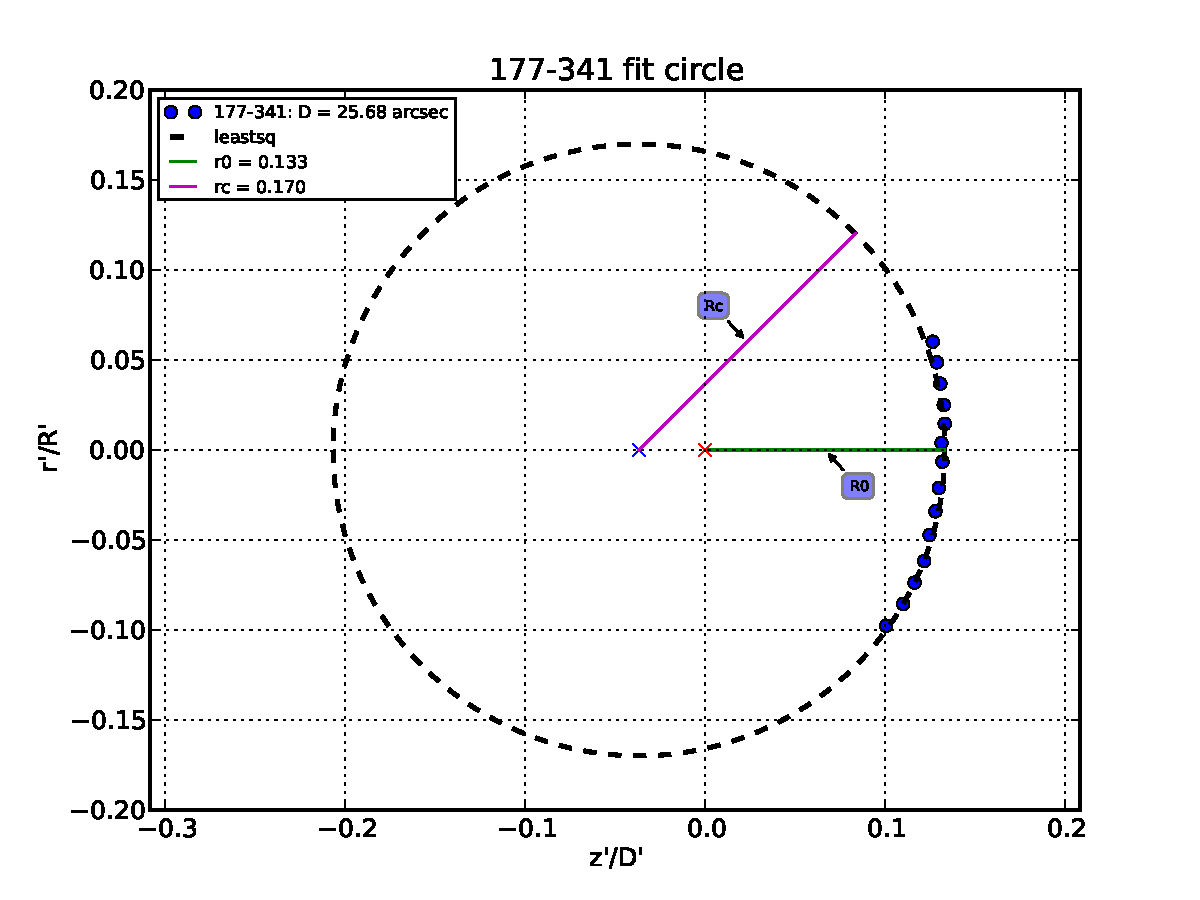
\includegraphics[width=0.5\linewidth]{LV-bowshocks-xyfancy-onaxis-502epositions-177-341}\\
%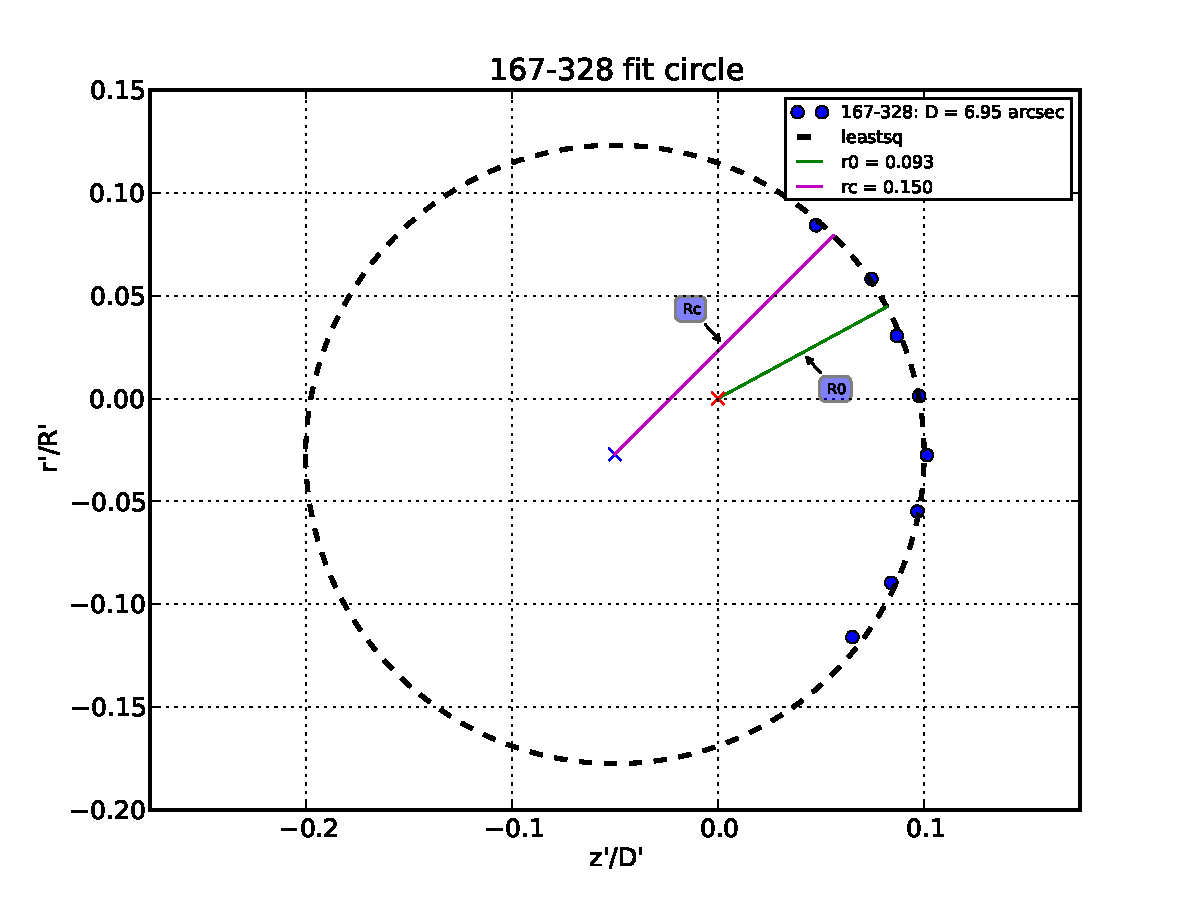
\includegraphics[width=0.5\linewidth]{LV-bowshocks-xyfancy-OIII3a-167-328} & 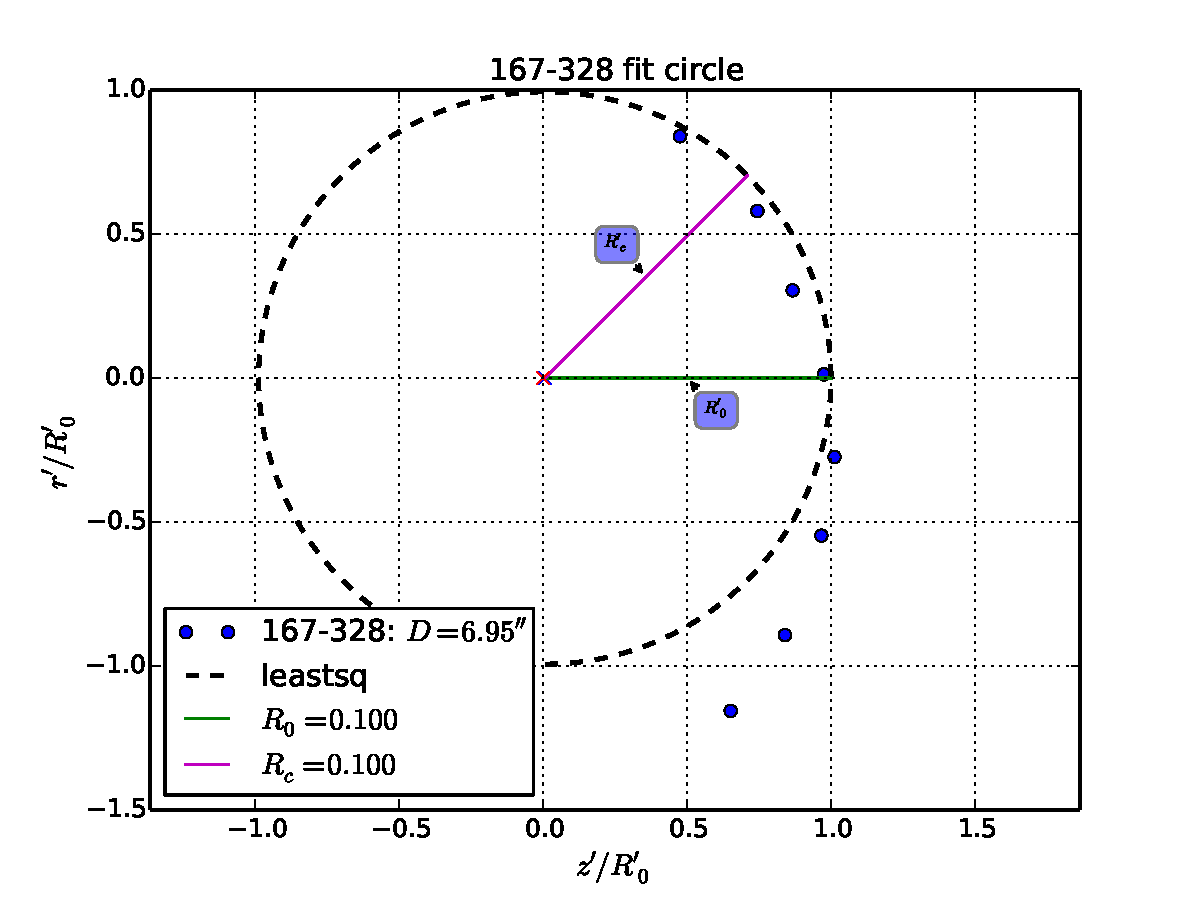
\includegraphics[width=0.5\linewidth]{LV-bowshocks-xyfancy-onaxis-OIII3a-167-328}
%\end{tabular}
%\label{fig:char-radii-obs-2}
%\caption{Continuation of figure (\ref{fig:char-radii-obs})}
%\end{figure*}
%
%\begin{figure*}
%\begin{tabular}{cc}
%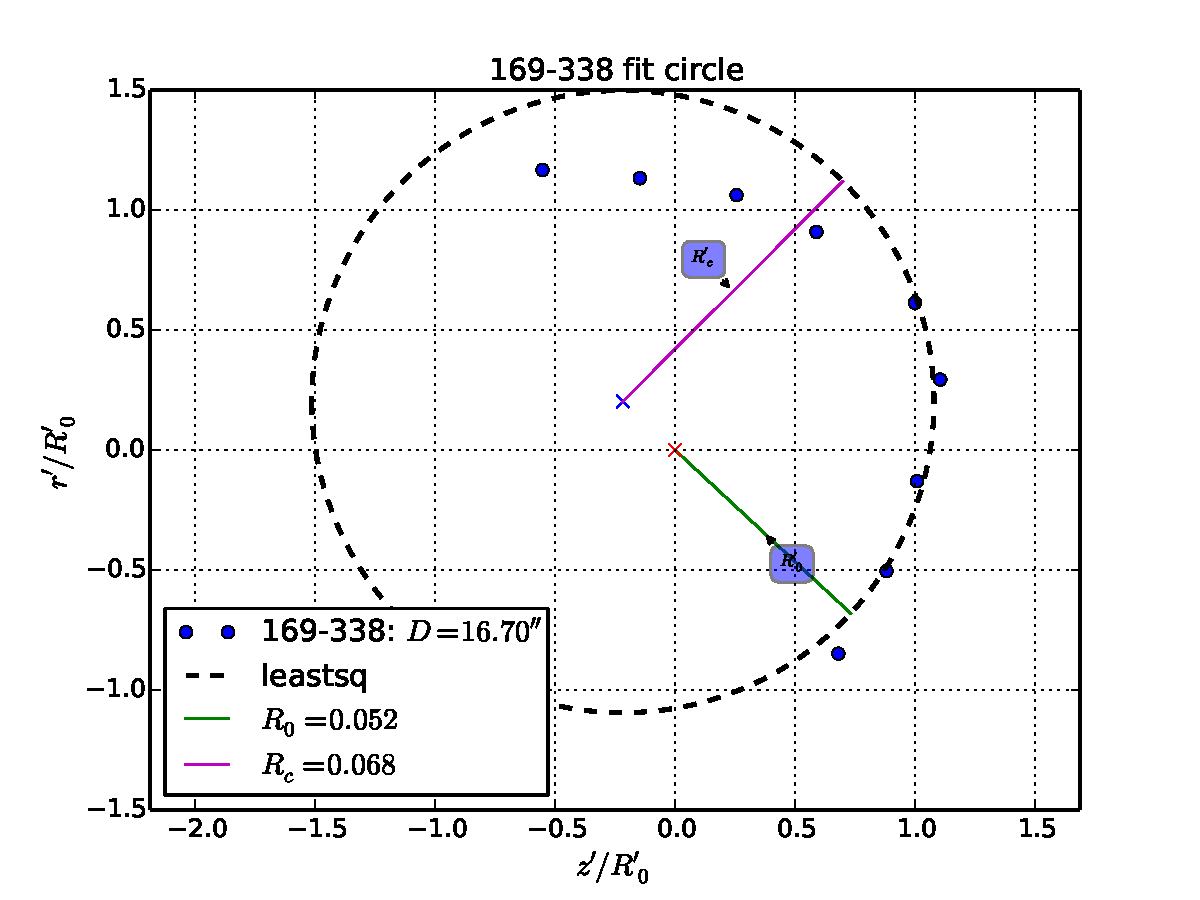
\includegraphics[width=0.5\linewidth]{LV-bowshocks-xyfancy-OIII3b-169-338} & 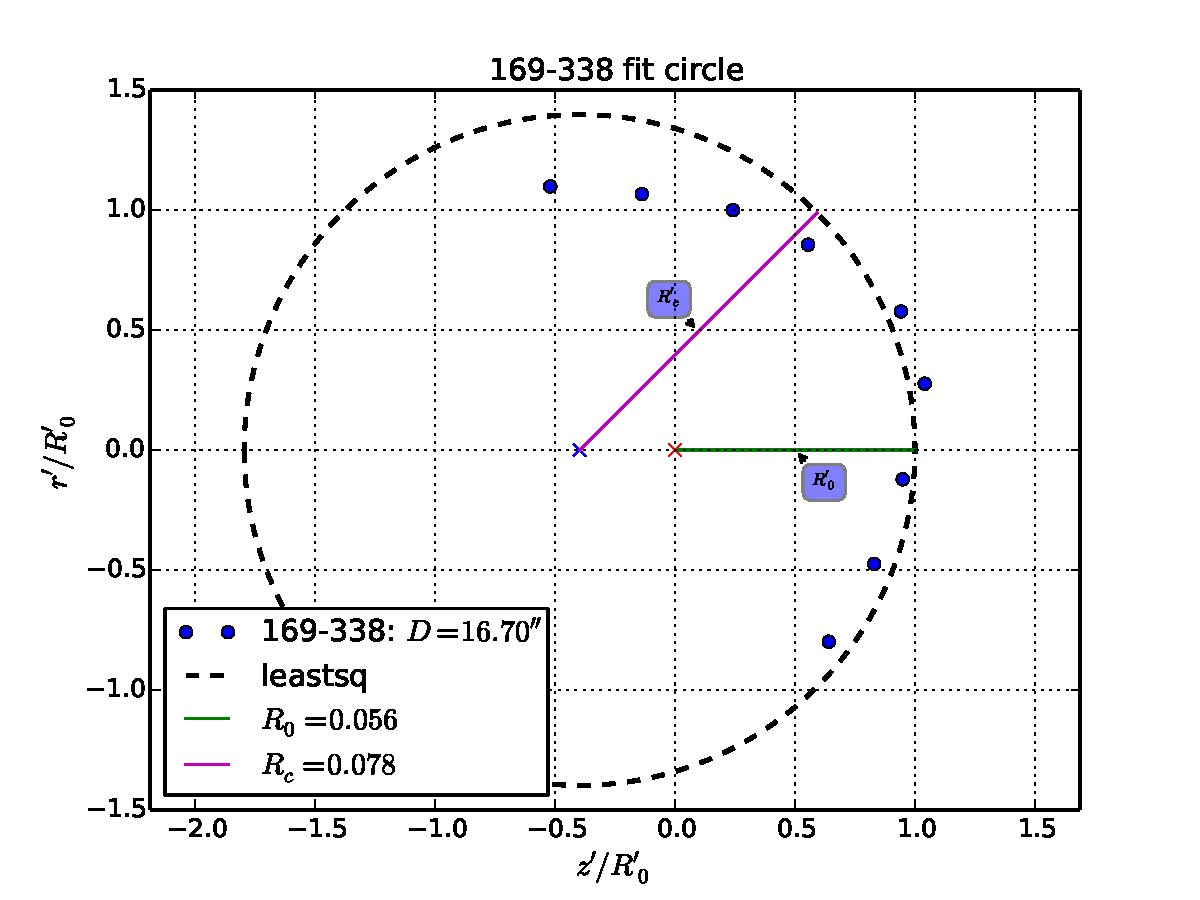
\includegraphics[width=0.5\linewidth]{LV-bowshocks-xyfancy-onaxis-OIII3b-169-338} \\
%\includegraphics[width=0.5\linewidth]{LV-bowshocks-xyfancy-OIII3b-189-329} & 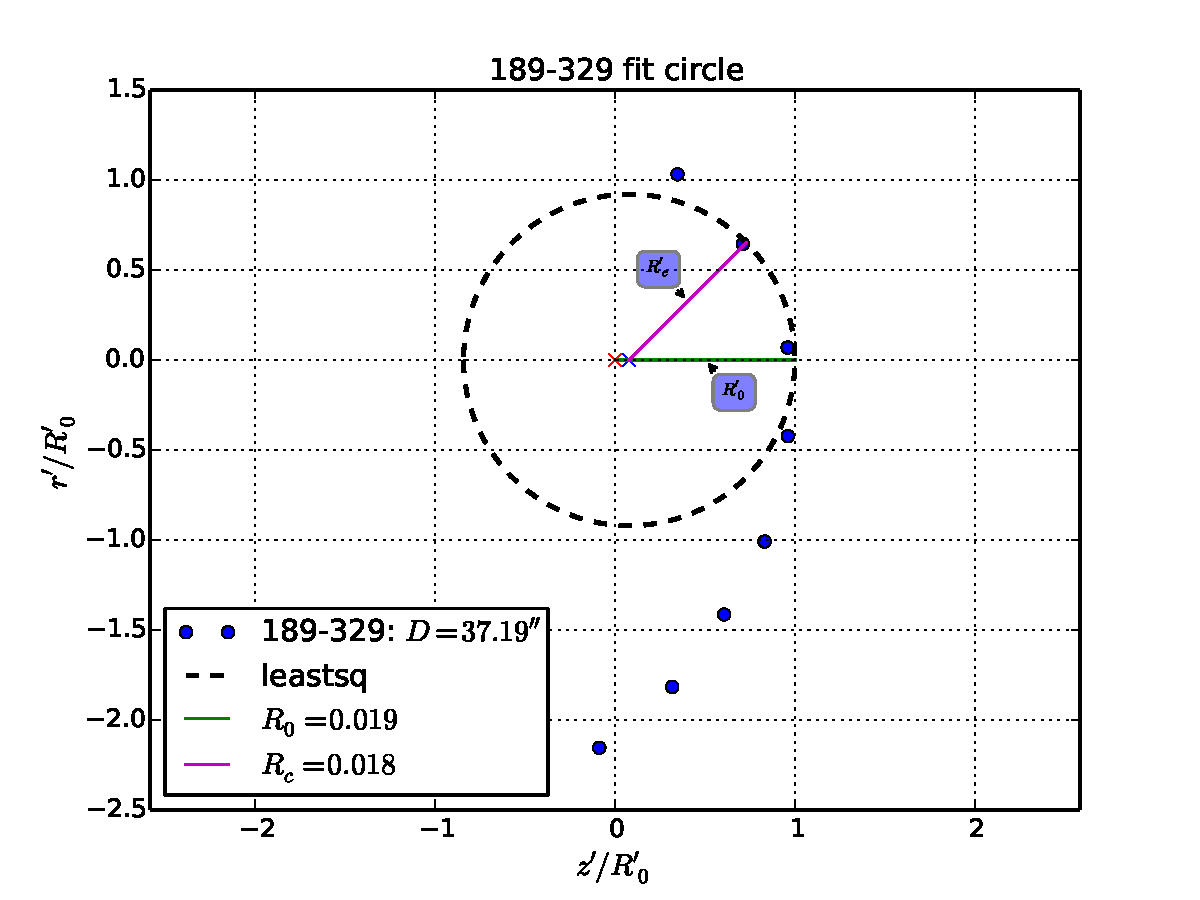
\includegraphics[width=0.5\linewidth]{LV-bowshocks-xyfancy-onaxis-OIII3b-189-329}\\
%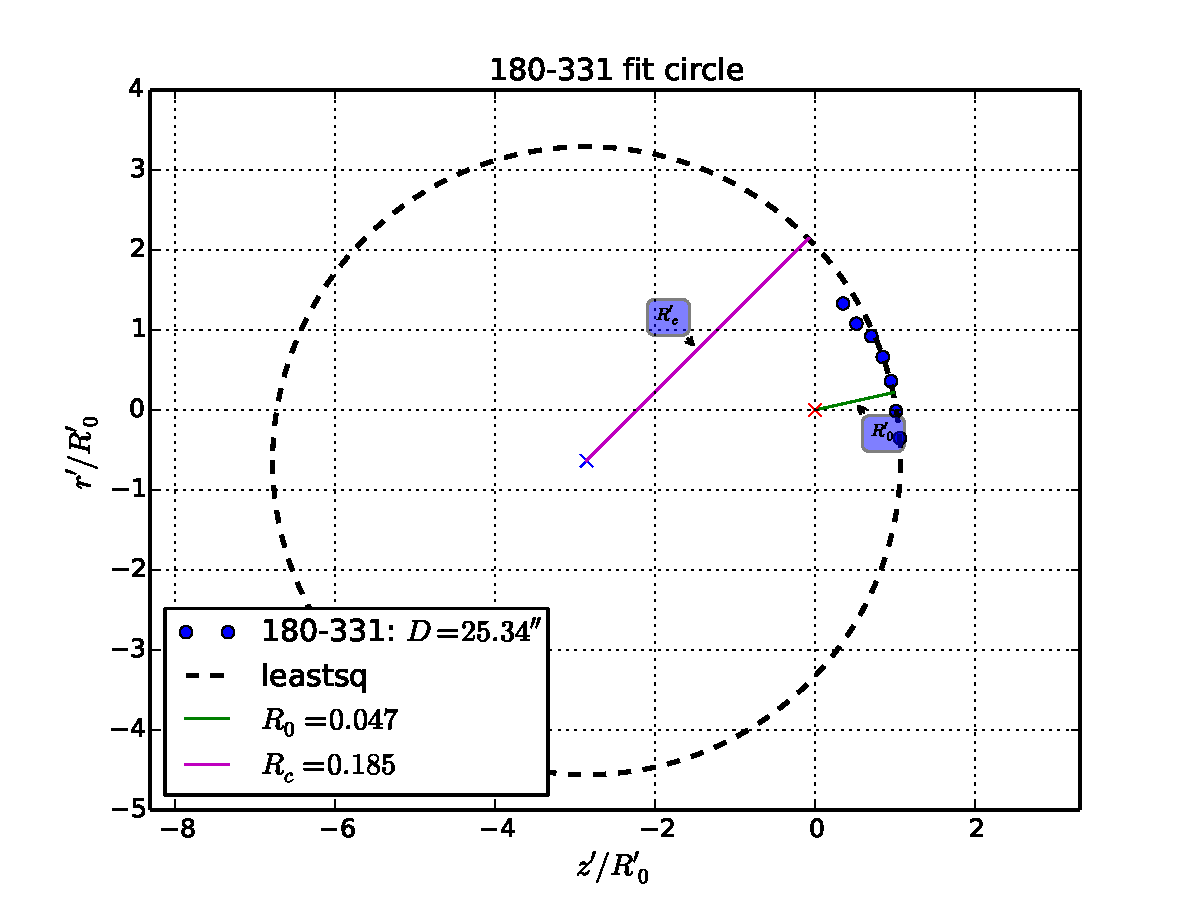
\includegraphics[width=0.5\linewidth]{LV-bowshocks-xyfancy-OIII3a-180-331} & 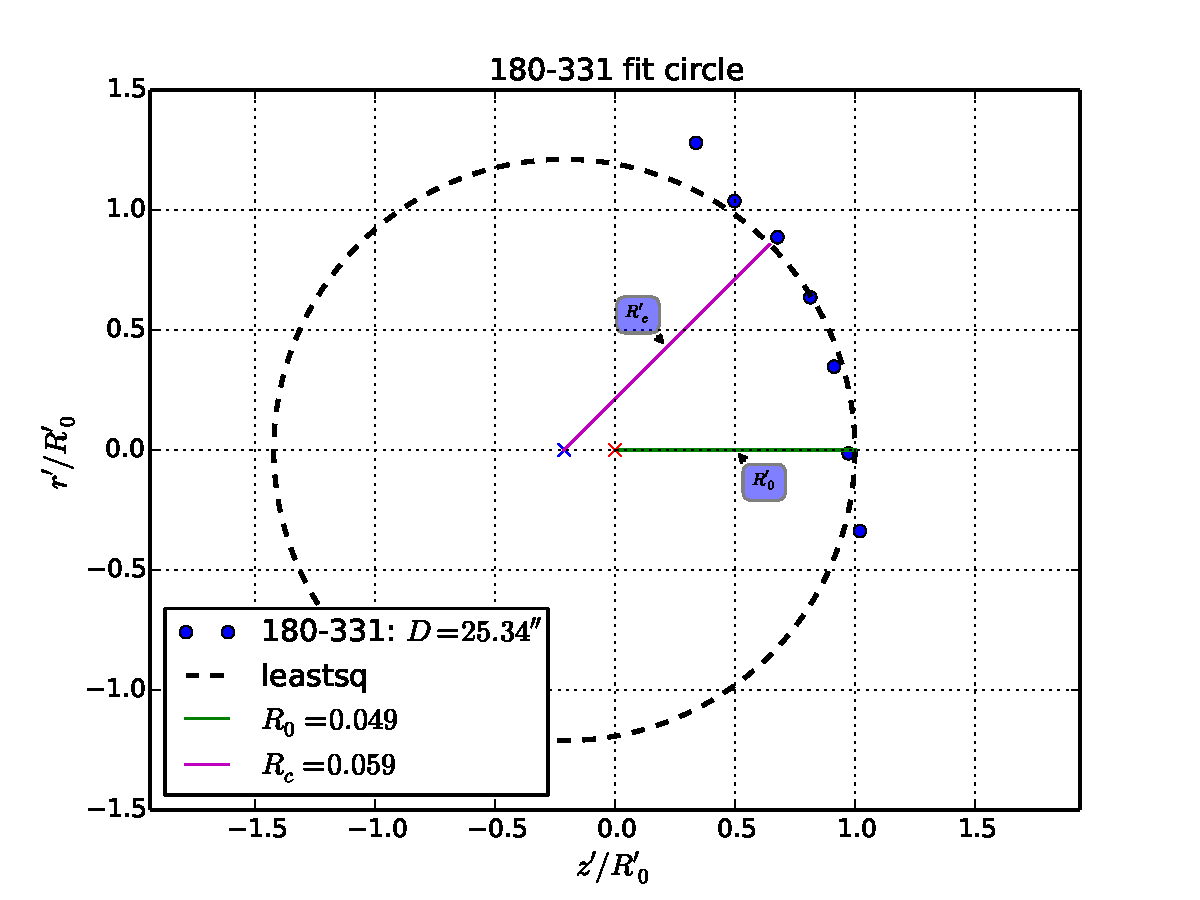
\includegraphics[width=0.5\linewidth]{LV-bowshocks-xyfancy-onaxis-OIII3a-180-331}
%\end{tabular}
%\label{fig:char-radii-obs-3}
%\caption{Continuation of figure (\ref{fig:char-radii-obs}), (new sample)}
%\end{figure*}


%%% Local Variables:
%%% mode: latex
%%% TeX-master: "proplyd-bowshocks"
%%% End:
